\documentclass[11pt,a4paper]{article}
\usepackage[margin=20mm]{geometry}
\usepackage{enumitem}
\usepackage{xcolor}
\usepackage{booktabs}
\usepackage{longtable}
\usepackage{array}
\usepackage{titlesec}
\usepackage{graphicx}
\usepackage{float}
\usepackage{caption}
\usepackage{listings}
\usepackage{tikz}
\usetikzlibrary{positioning,shapes.geometric,arrows.meta,fit,backgrounds,calc,decorations.pathreplacing}
\PassOptionsToPackage{hyphens}{url}
\usepackage[hidelinks]{hyperref}
\sloppy
\emergencystretch=3em
\Urlmuskip=0mu plus 3mu\relax

\graphicspath{{figures/}}

\definecolor{accent}{HTML}{1F6FB2}
\definecolor{soft}{HTML}{EEF4FA}
\definecolor{warn}{HTML}{B8860B}
\definecolor{good}{HTML}{2E7D32}
\definecolor{bad}{HTML}{C62828}
\titleformat{\section}{\Large\bfseries\color{accent}}{\thesection}{0.6em}{}
\titleformat{\subsection}{\large\bfseries}{\thesubsection}{0.5em}{}
\titleformat{\subsubsection}{\normalsize\bfseries}{\thesubsubsection}{0.5em}{}
\setlist[itemize]{leftmargin=1.4em,itemsep=2pt,topsep=3pt}
\setlength{\parindent}{0pt}
\setlength{\parskip}{5pt}

\lstset{basicstyle=\ttfamily\scriptsize,breaklines=true,frame=single,
  rulecolor=\color{accent},backgroundcolor=\color{soft},columns=fullflexible,
  keepspaces=true,showstringspaces=false,xleftmargin=2pt,xrightmargin=2pt}

\newcommand{\keynum}[2]{\textbf{#1} & #2 \\}
\tikzset{
  box/.style={rectangle,draw=accent,fill=soft,rounded corners=2pt,
    align=center,inner sep=4pt,font=\footnotesize,minimum height=8mm},
  dec/.style={diamond,draw=accent,fill=soft,align=center,inner sep=1pt,
    font=\scriptsize,aspect=2},
  fl/.style={-{Stealth[length=2mm]},draw=accent!80,thick},
}

\begin{document}

\begin{titlepage}
\centering
\vspace*{2.5cm}
{\Huge\bfseries NIDS}\\[6pt]
{\LARGE System Field Guide \& AI Roadmap}\\[18pt]
{\large A plain-English tour of every part of the dashboard,\\
the attacks it can and cannot see, and where it should go next}\\[2cm]
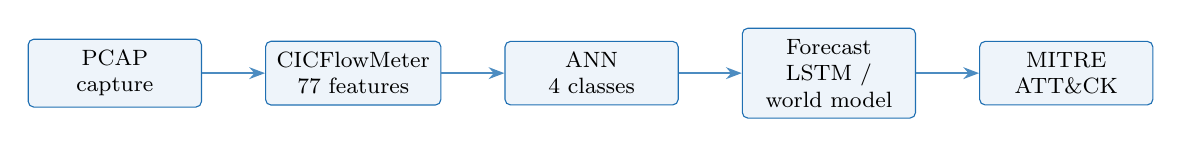
\begin{tikzpicture}
  \node[box,minimum width=22mm] (a) {PCAP\\capture};
  \node[box,minimum width=22mm,right=8mm of a] (b) {CICFlow\-Meter\\77 features};
  \node[box,minimum width=22mm,right=8mm of b] (c) {ANN\\4 classes};
  \node[box,minimum width=22mm,right=8mm of c] (d) {Forecast\\LSTM /\\world model};
  \node[box,minimum width=22mm,right=8mm of d] (e) {MITRE\\ATT\&CK};
  \draw[fl] (a)--(b); \draw[fl] (b)--(c); \draw[fl] (c)--(d); \draw[fl] (d)--(e);
\end{tikzpicture}
\vfill
{\small Generated \today\\ Offline system --- no cloud, no telemetry, no external call at inference time}
\end{titlepage}

\tableofcontents
\clearpage

\section*{How to read this document}
\addcontentsline{toc}{section}{How to read this document}

This guide has six parts.

\begin{itemize}
\item \textbf{Part I} explains what the system does \emph{today}, one stage at a
  time, in language a non-technical reader can follow. Each stage has a picture
  of the real dashboard and a small flow diagram.
\item \textbf{Part II} is a reference table of every function in the code, one
  line each, so an engineer can find the exact place a thing happens.
\item \textbf{Part III} lists the network attacks that exist and shows, for each,
  how this app can \emph{flag} it, \emph{predict} it, and \emph{prevent} it ---
  and honestly marks what it cannot do yet.
\item \textbf{Part IV} looks at real attacks that hit Indian organisations and
  what was done about them.
\item \textbf{Part V} surveys the 2026 open-source and AI landscape --- the
  projects that have already solved large parts of this problem.
\item \textbf{Part VI} is the recommended plan: adopt the solved pieces, keep our
  forecasting engine as the thing that is genuinely new.
\end{itemize}

A one-line summary of the system: \emph{it watches network traffic, decides
whether the traffic looks like an attack, predicts what the next few seconds
look like, and explains its reasoning against the MITRE ATT\&CK catalogue ---
all on one machine, with nothing sent anywhere.}

\clearpage
\part*{Part I --- What NIDS does today}
\addcontentsline{toc}{section}{PART I --- What NIDS does today}

\section{The big picture}

Network defence usually labels each ``flow'' (one conversation between two
computers) as good or bad and stops there. That throws away \emph{time} --- the
order in which an attacker probes ports, the way a burst of half-open
connections comes before a flood, the reconnaissance that happens before
lateral movement. NIDS keeps the time dimension: it rolls flows up into
10-second windows, learns how the ``state'' of the network moves from one window
to the next, and forecasts the next few windows.

\begin{figure}[H]
\centering
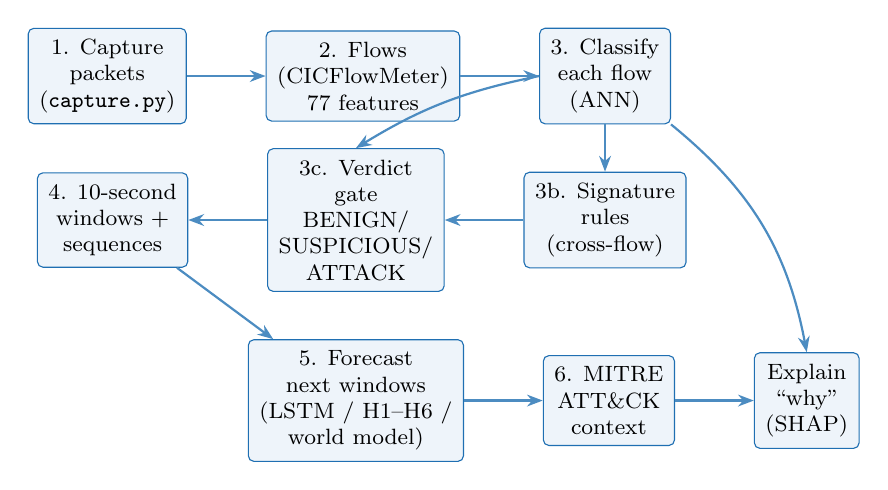
\begin{tikzpicture}[node distance=6mm and 10mm]
  \node[box] (cap) {1. Capture\\packets\\(\texttt{capture.py})};
  \node[box,right=of cap] (ext) {2. Flows\\(CICFlowMeter)\\77 features};
  \node[box,right=of ext] (ann) {3. Classify\\each flow\\(ANN)};
  \node[box,below=of ann] (sig) {3b. Signature\\rules\\(cross-flow)};
  \node[box,left=of sig] (ver) {3c. Verdict\\gate\\BENIGN/\\SUSPICIOUS/\\ATTACK};
  \node[box,left=of ver] (tmp) {4. 10-second\\windows +\\sequences};
  \node[box,below=of ver] (fc) {5. Forecast\\next windows\\(LSTM / H1--H6 /\\world model)};
  \node[box,right=of fc] (mit) {6. MITRE\\ATT\&CK\\context};
  \node[box,right=of mit] (exp) {Explain\\``why''\\(SHAP)};
  \draw[fl] (cap)--(ext); \draw[fl] (ext)--(ann); \draw[fl] (ann)--(sig);
  \draw[fl] (ann.west) to[bend right=10] (ver.north);
  \draw[fl] (sig)--(ver); \draw[fl] (ver)--(tmp); \draw[fl] (tmp)--(fc);
  \draw[fl] (fc)--(mit); \draw[fl] (mit)--(exp);
  \draw[fl] (ann.south east) to[bend left=20] (exp.north);
\end{tikzpicture}
\caption{The whole pipeline. Everything runs locally; each arrow is a step a
person or a timer triggers.}
\end{figure}

\textbf{The pipeline in one paragraph.} Raw packets are recorded to a
\texttt{.pcap} file. CICFlowMeter turns that file into a table of flows, one row
per conversation, each row summarised by 77 numbers (packet counts, byte totals,
timing statistics, TCP-flag counts). A small neural network (the ANN) scores
every flow as \texttt{BENIGN}, \texttt{DDoS}, \texttt{DoS} or \texttt{PortScan}.
A separate rule layer looks across \emph{all} flows at once to catch volumetric
floods the per-flow view dilutes. A ``verdict gate'' decides whether the whole
capture reads green (BENIGN), amber (SUSPICIOUS) or red (ATTACK). The labelled
flows are then rolled into 10-second windows; a forecasting model predicts the
next window's state (and a longer model predicts the next six). Finally a
deterministic mapper attaches MITRE ATT\&CK technique candidates and an
operator playbook, and a feature-attribution step explains which inputs drove
the call.

\begin{table}[H]\centering\small
\begin{tabular}{@{}ll@{}}
\toprule
\textbf{Fact} & \textbf{Value} \\
\midrule
\keynum{Attack classes}{BENIGN, DDoS, DoS, PortScan (4-way softmax)}
\keynum{Flow features}{77 (CICFlowMeter / CICIDS2017 schema)}
\keynum{Window length}{10 seconds (real timestamps, temporal pipeline)}
\keynum{Sequence length}{5 windows in $\rightarrow$ 1 window out}
\keynum{Forecast horizons}{1 window; also direct H1--H6; world model K=6 (max 24)}
\keynum{Verdict gate}{a class reads red only if its own share of flows $\geq$ 20\%}
\keynum{Deployment}{single machine, offline, FastAPI + static dashboard on \texttt{:8765}}
\bottomrule
\end{tabular}
\caption{The numbers that matter most, collected here and in Appendix~B.}
\end{table}

\begin{figure}[H]\centering
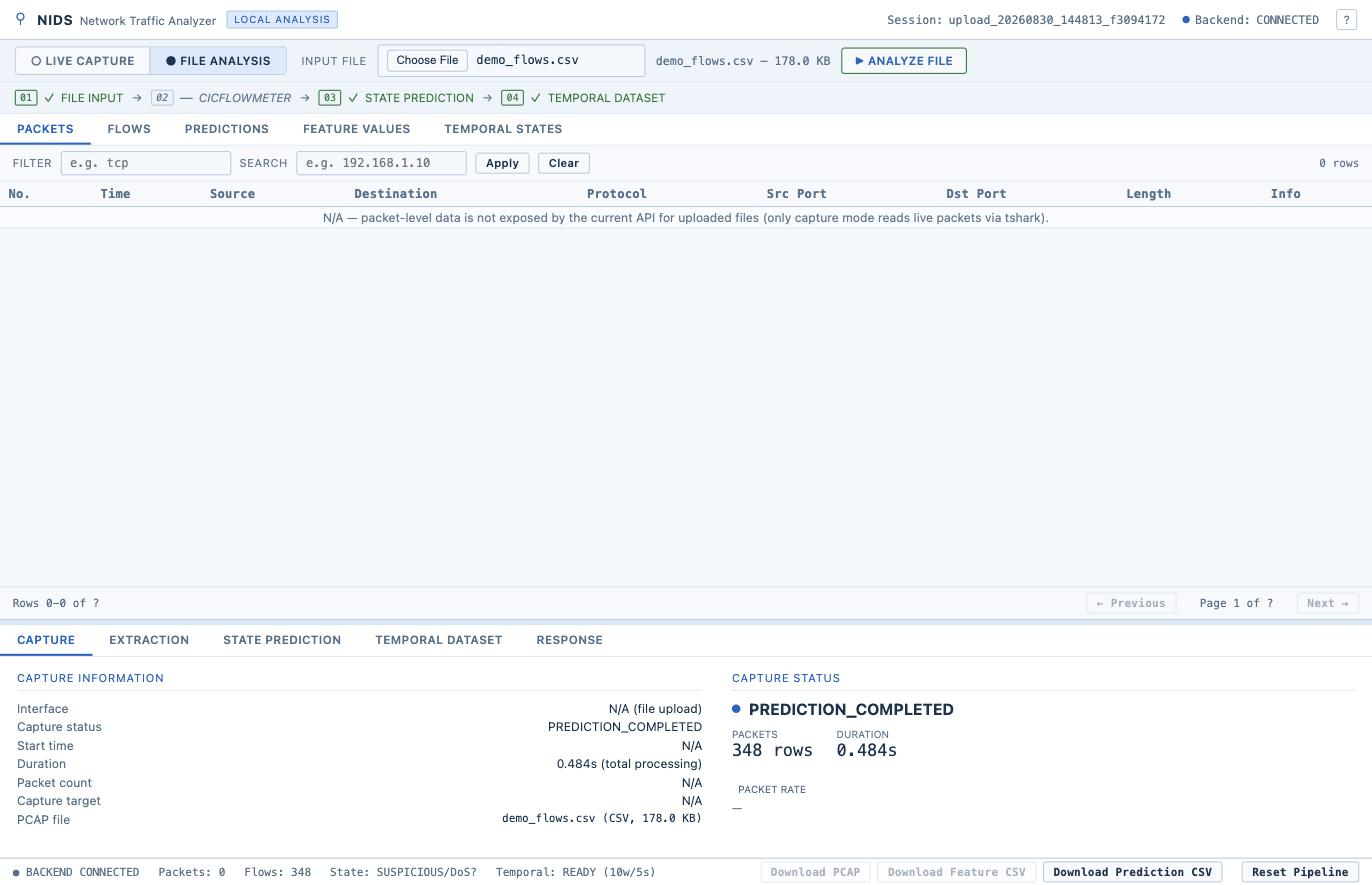
\includegraphics[width=\linewidth]{fig-overview-fileanalysis.jpg}
\caption{The dashboard after analysing a capture. Top strip: the four pipeline
stages. Left: a table of packets / flows / predictions. Right: detail panels.
Bottom bar: live counters and the current verdict.}
\end{figure}

\section{Stage 1 --- Capturing packets}

\subsection*{What it does, in plain words}
\begin{itemize}
\item Records live network traffic to a \texttt{.pcap} file, the standard format
  every analysis tool understands.
\item Uses the operating system's own capture tool --- \texttt{dumpcap} on
  Windows, \texttt{tcpdump} on macOS/Linux --- started as a child process.
\item Never invents numbers. The packet count shown is read back from the file
  by \texttt{capinfos} after the capture stops; while running it re-reads the
  growing file.
\item Has three ways to stop: a duration target (default 300\,s), an optional
  packet target, and a hard safety timeout at 600\,s so a forgotten capture
  cannot fill the disk.
\item Drains the capture tool's error output on a background thread so a full
  OS pipe buffer cannot freeze the capture, and keeps the last 200 lines for
  diagnostics.
\end{itemize}

\begin{figure}[H]\centering
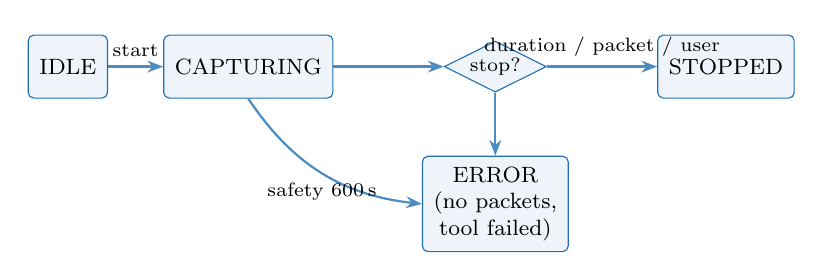
\begin{tikzpicture}[node distance=5mm and 7mm]
  \node[box] (i) {IDLE};
  \node[box,right=of i] (c) {CAPTURING};
  \node[dec,right=14mm of c] (d) {stop?};
  \node[box,right=14mm of d] (s) {STOPPED};
  \node[box,below=8mm of d] (e) {ERROR\\(no packets,\\tool failed)};
  \draw[fl] (i)--node[above,font=\scriptsize]{start} (c);
  \draw[fl] (c)--(d);
  \draw[fl] (d)--node[above,font=\scriptsize]{duration / packet / user} (s);
  \draw[fl] (d)--(e);
  \draw[fl] (c.south) to[bend right=25] node[below,font=\scriptsize]{safety 600\,s} (e.west);
\end{tikzpicture}
\caption{Capture state machine (\texttt{capture.py}). \texttt{check\_and\_finalize()}
runs on every status poll and is the only place the duration and safety limits
are enforced.}
\end{figure}

\begin{table}[H]\centering\small
\begin{tabular}{@{}ll@{}}
\toprule
\textbf{Setting} & \textbf{Default} \\ \midrule
\keynum{Capture duration}{300 s}
\keynum{Packet target}{none (a flood is not cut short in a fraction of a second)}
\keynum{Kernel buffer}{64 MiB}
\keynum{Safety timeout}{600 s}
\keynum{Packet-table page size}{100 rows; hard ceiling 50\,000 per read}
\bottomrule
\end{tabular}
\caption{Capture defaults, from \texttt{backend/capture/capture.py}.}
\end{table}

\begin{figure}[H]\centering
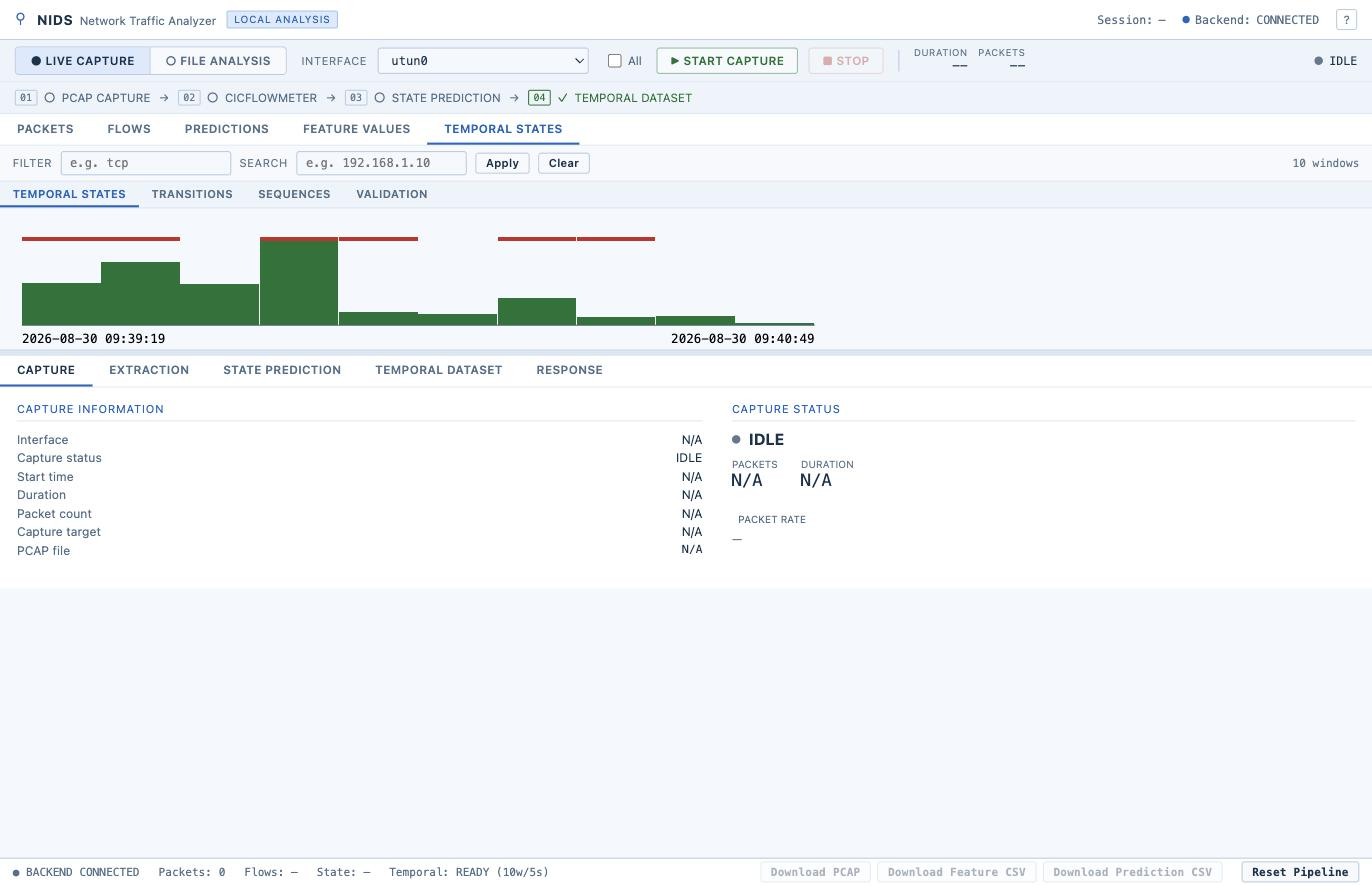
\includegraphics[width=0.92\linewidth]{fig-live-capture.jpg}
\caption{The live-capture panel before a run. Interface picker, Start/Stop,
duration and packet counters, and a live packets-per-second sparkline once a
capture is running.}
\end{figure}

\section{Stage 2 --- Turning packets into flows (CICFlowMeter)}

\subsection*{What a ``flow'' is}
A flow is one two-way conversation between two computers, identified by five
things: source IP, destination IP, source port, destination port, and protocol.
CICFlowMeter reads the whole capture once and, for each flow, produces one row
of about 80 columns --- packet counts each direction, byte totals,
inter-arrival-time mean/standard-deviation/min/max, TCP-flag counts, header
lengths, packet-length statistics, bytes-per-second and packets-per-second,
active/idle times. The ANN uses 77 of those columns (the exact CICIDS2017
training schema in \texttt{features.py}).

\begin{itemize}
\item Uses the \texttt{cicflowmeter} Python package (a drop-in for the original
  Java tool). Two upstream bugs are patched once by
  \texttt{scripts/patch\_cicflowmeter.py}.
\item Large captures are split on packet boundaries with \texttt{editcap} into
  20\,000-packet chunks and processed in parallel, then the per-chunk CSVs are
  concatenated. A flow that straddles a cut is counted once per chunk --- a
  small, documented inflation the large chunk size keeps rare.
\item Column names drift between CICFlowMeter versions. \texttt{match\_columns()}
  aligns any naming style to the 77 training features by reducing each name to a
  set of canonical tokens (so ``Total Fwd Packets'' and ``Tot Fwd Pkts'' match).
  It raises rather than silently misalign.
\end{itemize}

\begin{figure}[H]\centering
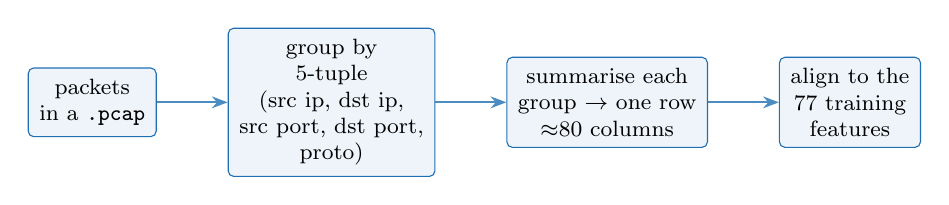
\begin{tikzpicture}[node distance=5mm and 9mm]
  \node[box] (p) {packets\\in a \texttt{.pcap}};
  \node[box,right=of p] (g) {group by\\5-tuple\\(src ip, dst ip,\\src port, dst port,\\proto)};
  \node[box,right=of g] (a) {summarise each\\group $\rightarrow$ one row\\$\approx$80 columns};
  \node[box,right=of a] (m) {align to the\\77 training\\features};
  \draw[fl] (p)--(g); \draw[fl] (g)--(a); \draw[fl] (a)--(m);
\end{tikzpicture}
\caption{Flow extraction. One conversation becomes one row of numbers.}
\end{figure}

\begin{figure}[H]\centering
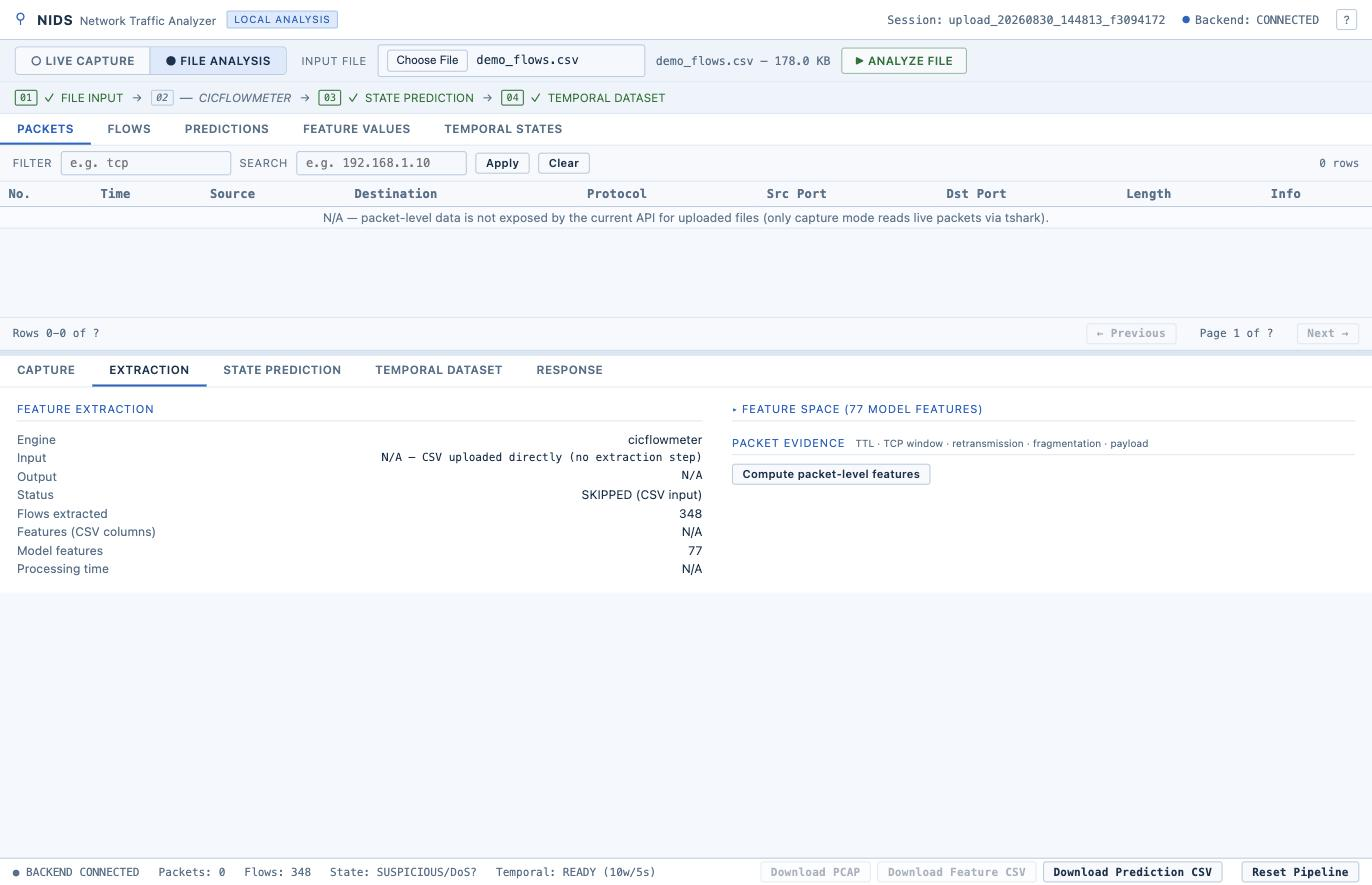
\includegraphics[width=0.92\linewidth]{fig-extraction.jpg}
\caption{The extraction panel. For an uploaded CSV this step is skipped (the
rows are already flows); for a capture it shows flow count, feature count and
processing time. ``Feature space'' lists the 77 model features; ``Packet
evidence'' is the separate Scapy pass below.}
\end{figure}

\subsection{Stage 2b --- Packet-level evidence}
A second, independent pass (\texttt{packet\_features.py}, using Scapy) reads the
capture directly and computes per-flow \emph{packet}-level signals that flow
statistics miss: TTL mean/spread, TCP window behaviour, retransmission count,
IP-fragment count, payload-length statistics. It also classifies port-scan
\emph{order} --- whether destination ports were walked \texttt{sequential},
\texttt{strided} or \texttt{randomised}. None of this feeds the ANN; it is
shown as corroborating evidence on the dashboard.

\section{Stage 3 --- The neural-network classifier}

\subsection*{What it does, in plain words}
\begin{itemize}
\item Loads a pre-trained Keras model (\texttt{ISAA\_ANN.h5}, a small
  multi-layer network) and its scaler (\texttt{minmax.bin}).
\item Scales every flow's 77 features to the 0--1 range the model was trained
  on, then asks the model for four probabilities that sum to 1: how
  \texttt{BENIGN}, \texttt{DDoS}, \texttt{DoS}, \texttt{PortScan} the flow looks.
\item The largest probability is the flow's label; the probability itself is the
  ``confidence''.
\item A flow whose features contain infinities or gaps (a known CICFlowMeter
  artefact for zero-duration flows) is never guessed --- it is marked
  \texttt{INVALID\_FEATURES} and excluded from scoring.
\item The labels are written back onto the CSV as three new columns
  (\texttt{Current\_State} = the ANN call, \texttt{Signature\_State} = the rule
  layer's call, \texttt{Effective\_State} = the merged call) so the file and the
  on-screen numbers can never disagree.
\end{itemize}

\begin{figure}[H]\centering
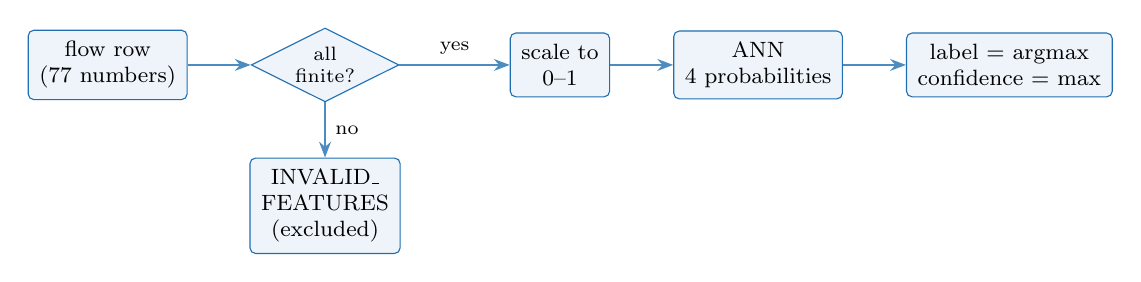
\begin{tikzpicture}[node distance=4.5mm and 8mm]
  \node[box] (r) {flow row\\(77 numbers)};
  \node[dec,right=of r] (v) {all\\finite?};
  \node[box,below=7mm of v] (inv) {INVALID\_\\FEATURES\\(excluded)};
  \node[box,right=14mm of v] (s) {scale to\\0--1};
  \node[box,right=of s] (n) {ANN\\4 probabilities};
  \node[box,right=of n] (o) {label = argmax\\confidence = max};
  \draw[fl] (r)--(v); \draw[fl] (v)--node[above,font=\scriptsize]{yes}(s);
  \draw[fl] (v)--node[right,font=\scriptsize]{no}(inv);
  \draw[fl] (s)--(n); \draw[fl] (n)--(o);
\end{tikzpicture}
\caption{Per-flow scoring (\texttt{predict.py}).}
\end{figure}

\subsection{Stage 3b --- The signature layer}
The ANN sees one flow at a time, so a volumetric DDoS --- thousands of small,
individually-innocuous flows --- can be diluted to ``mostly BENIGN''. The
signature layer (\texttt{signatures.py}) looks across the whole flow table at
once and fires three deterministic rules:

\begin{table}[H]\centering\small
\begin{tabular}{@{}p{3cm}p{7.5cm}p{3.5cm}@{}}
\toprule
\textbf{Rule} & \textbf{Fires when} & \textbf{Marks} \\ \midrule
Rolling flood & in a 1-second bucket, one victim IP is hit by $\geq$20 distinct
  sources, that victim holds $\geq$50\% of the window's flows, the busiest single
  source is $\leq$25\% of them, and packet rate $\geq$100/s & every flow in the
  group $\rightarrow$ \texttt{DDoS} \\
SYN / half-open flood & a flow has $\geq$20 SYNs, ACK/SYN $\leq$0.2, and
  $\geq$100 packets/s & BENIGN rows $\rightarrow$ \texttt{DoS} \\
Port sweep & one source contacts $\geq$20 distinct destination ports on one
  destination with mean forward bytes $\leq$400 & BENIGN rows $\rightarrow$
  \texttt{PortScan} \\
\bottomrule
\end{tabular}
\caption{Signature rules. This layer never overwrites a real ANN call --- it
only relabels flows the ANN left \texttt{BENIGN} or \texttt{INVALID\_FEATURES},
and it can clear the verdict gate for its class.}
\end{table}

\subsection{Stage 3c --- The verdict gate}
The headline a defender reads is one of three: green \textbf{BENIGN}, amber
\textbf{SUSPICIOUS}, red \textbf{ATTACK}. The gate
(\texttt{summarize\_states()}) decides which.

\begin{figure}[H]\centering
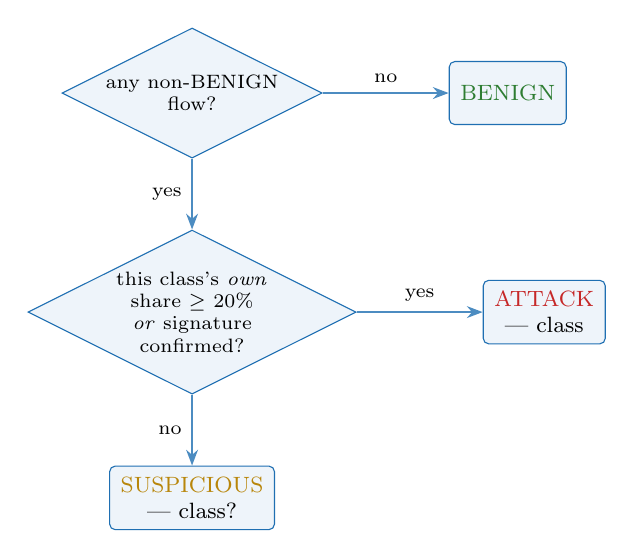
\begin{tikzpicture}[node distance=5mm and 10mm]
  \node[dec] (a) {any non-BENIGN\\flow?};
  \node[box,right=16mm of a] (b) {\color{good}BENIGN};
  \node[dec,below=9mm of a] (c) {this class's \emph{own}\\share $\geq$ 20\%\\\emph{or} signature\\confirmed?};
  \node[box,right=16mm of c] (d) {\color{bad}ATTACK\\--- class};
  \node[box,below=9mm of c] (e) {\color{warn}SUSPICIOUS\\--- class?};
  \draw[fl] (a)--node[above,font=\scriptsize]{no}(b);
  \draw[fl] (a)--node[left,font=\scriptsize]{yes}(c);
  \draw[fl] (c)--node[above,font=\scriptsize]{yes}(d);
  \draw[fl] (c)--node[left,font=\scriptsize]{no}(e);
\end{tikzpicture}
\caption{The verdict gate. The test is on the attack class's \emph{own}
percentage of scored flows --- so a minority DoS is not promoted to red by
unrelated DDoS flows in the same capture. Thresholds live in
\texttt{config/config.json} and can be retuned without touching code.}
\end{figure}

\begin{figure}[H]\centering
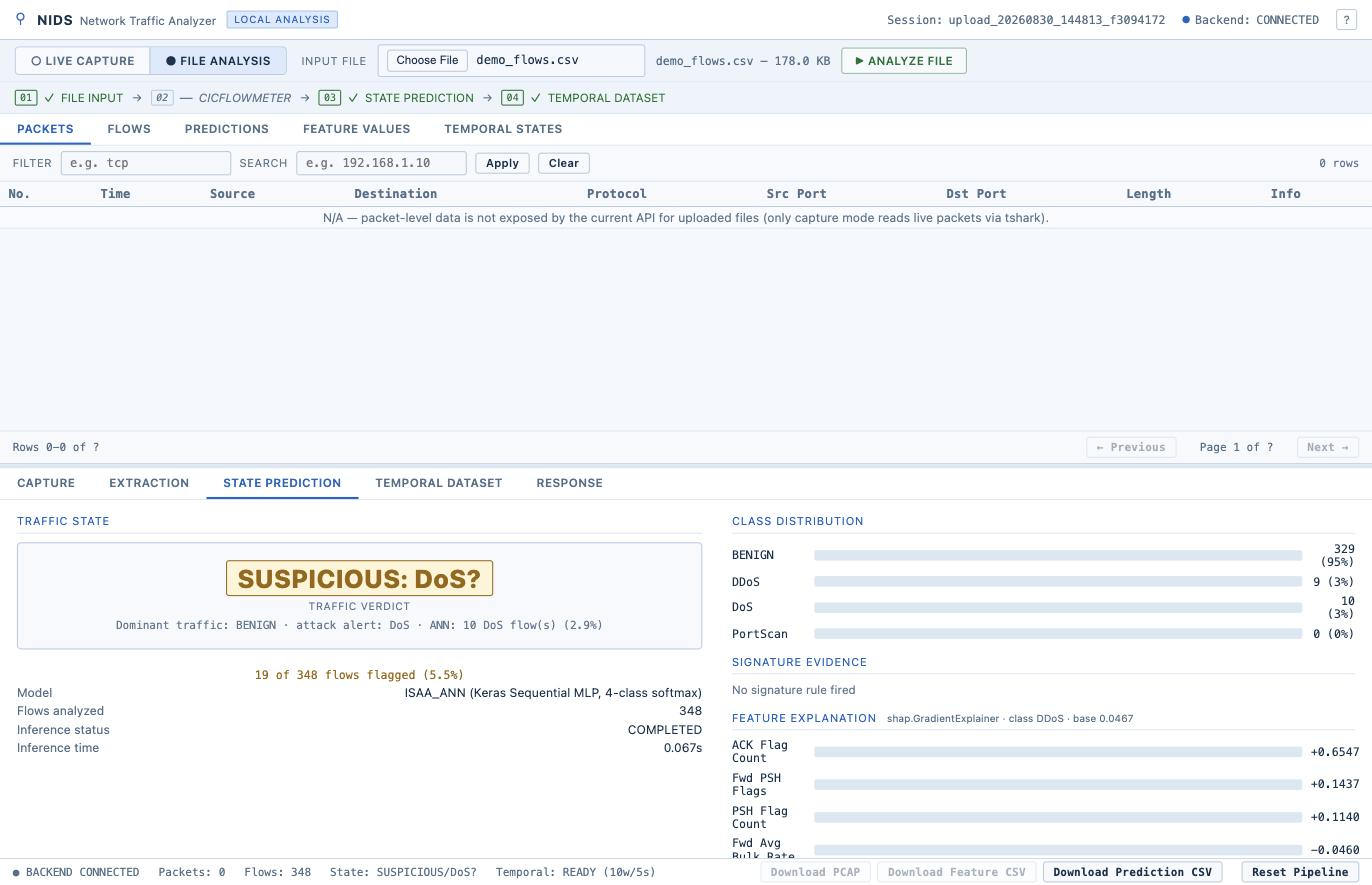
\includegraphics[width=\linewidth]{fig-verdict-hero.jpg}
\caption{A real verdict. This capture is 95\% benign with 10 DoS flows out of
348 (2.9\%). Because DoS's own share is well under 20\% and no signature fired,
the hero reads amber \textbf{SUSPICIOUS: DoS?}, not red. The class-distribution
bars, ``no signature rule fired'', and the SHAP feature explanation are all on
this one panel.}
\end{figure}

\subsection{Stage 3d --- Explaining a prediction}
Two mechanisms:
\begin{itemize}
\item \textbf{Always on:} a single gradient-times-input pass
  (\texttt{explain.py}) gives, per flow, how much each of the 77 features pushed
  the model toward its chosen class. The capture-wide top 10 are shown as
  ``driving features''.
\item \textbf{When a background sample exists:} real SHAP values
  (\texttt{shap\_service.py}) computed by an async job. The dashboard shows
  \texttt{shap.GradientExplainer} when SHAP ran and
  ``gradient\,$\times$\,input fallback --- not SHAP'' otherwise. The background
  file \texttt{models/ann\_shap\_background.npy} is present, so real SHAP runs.
\end{itemize}

\subsection{Stage 3e --- Classifier quality}
The metrics panel (\texttt{metrics.py}) reports precision, recall, F1 and support
per class, macro/weighted F1, accuracy, an attack-vs-benign block with false-
positive rate, and a 4$\times$4 confusion matrix. It uses \emph{real}
CICIDS2017 ground-truth labels when a labelled CSV directory is configured
(\texttt{NIDS\_CICIDS2017\_DIR}); otherwise it falls back to a \emph{proxy} ---
how often the ANN agrees with the signature layer --- and labels it clearly as
``PROXY (not ground truth)''.

\begin{figure}[H]\centering
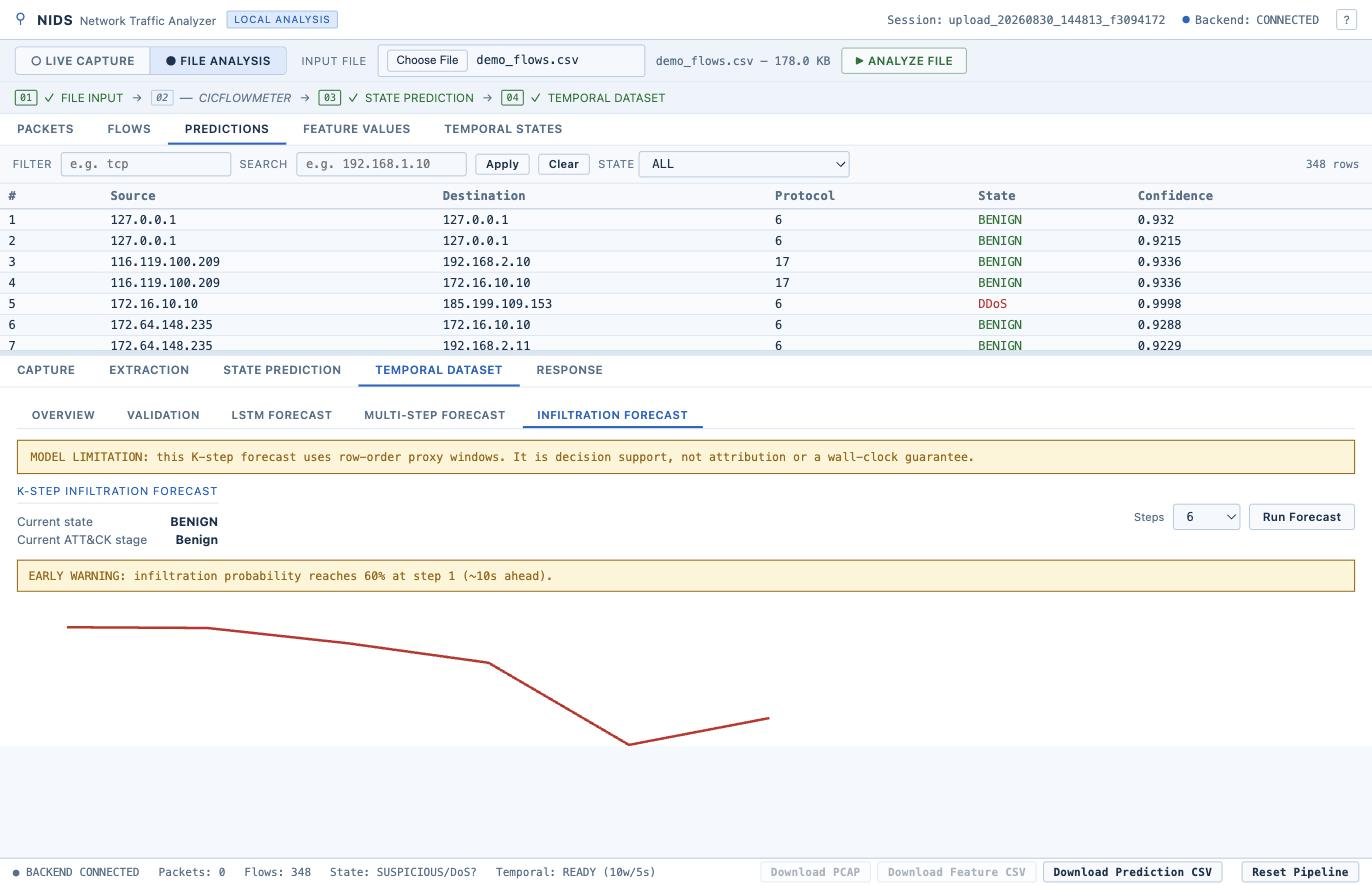
\includegraphics[width=\linewidth]{fig-predictions-table.jpg}
\caption{Per-flow predictions: source, destination, protocol, ANN state,
confidence. Row 5 here is a DDoS flow scored at 0.9998.}
\end{figure}

\begin{figure}[H]\centering
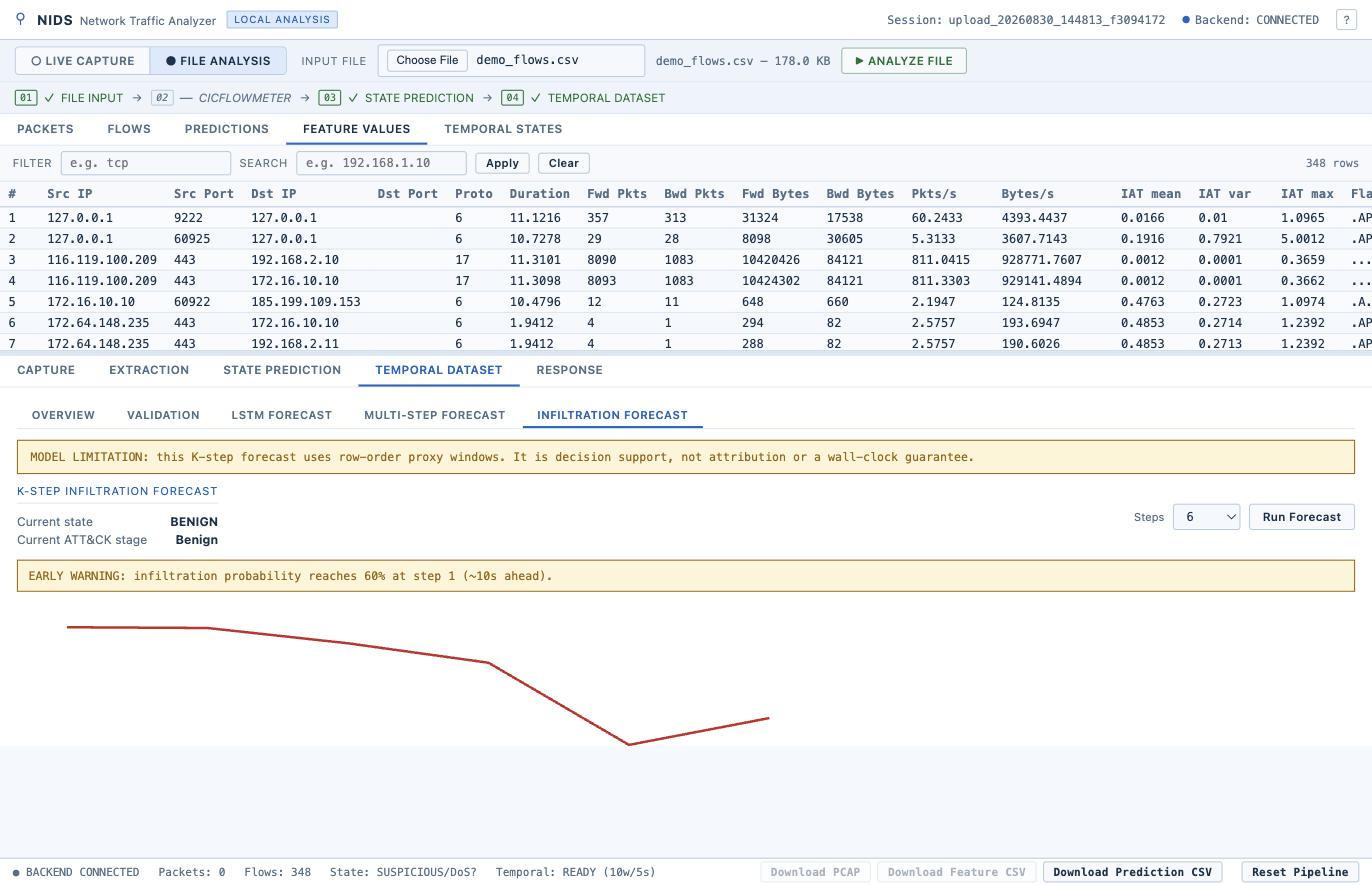
\includegraphics[width=\linewidth]{fig-featurevalues-table.jpg}
\caption{The raw feature values behind each flow --- duration, packet and byte
counts each direction, rates, inter-arrival timing, and the TCP-flag bitmask.}
\end{figure}

\section{Stage 4 --- Building the time-series dataset}

\subsection*{What it does, in plain words}
\begin{itemize}
\item Reads the labelled flow CSV, sorts by real timestamp, and slices time into
  fixed \textbf{10-second windows}.
\item For each window it computes a 28-number ``state vector'' --- flow count,
  unique source/destination IPs and ports, packet and byte totals and rates,
  TCP-flag totals, inter-arrival-time statistics --- plus the dominant class in
  that window and an \texttt{attack\_present} flag.
\item Builds a table of window-to-window transitions (with the real time gap
  between them, because empty windows are never invented).
\item Slides a length-5 window across the states: five consecutive state vectors
  are the input, the sixth window's state is the answer.
\item Splits the timeline \textbf{chronologically} 70/15/15 into train /
  validation / test --- never shuffled --- and fits the scaler on the training
  windows only.
\end{itemize}

\begin{figure}[H]\centering
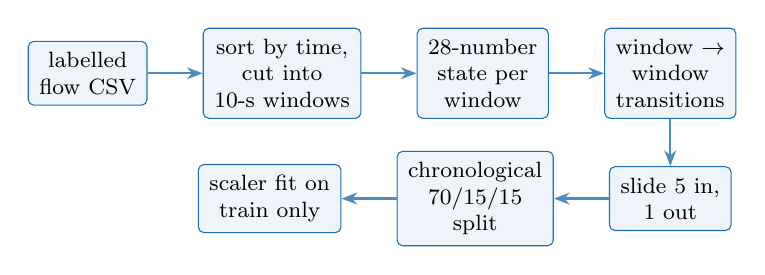
\begin{tikzpicture}[node distance=4mm and 7mm]
  \node[box] (c) {labelled\\flow CSV};
  \node[box,right=of c] (w) {sort by time,\\cut into\\10-s windows};
  \node[box,right=of w] (s) {28-number\\state per\\window};
  \node[box,right=of s] (t) {window $\to$\\window\\transitions};
  \node[box,below=6mm of t] (q) {slide 5 in,\\1 out};
  \node[box,left=of q] (p) {chronological\\70/15/15\\split};
  \node[box,left=of p] (sc) {scaler fit on\\train only};
  \draw[fl] (c)--(w); \draw[fl] (w)--(s); \draw[fl] (s)--(t);
  \draw[fl] (t)--(q); \draw[fl] (q)--(p); \draw[fl] (p)--(sc);
\end{tikzpicture}
\caption{Temporal dataset preparation (\texttt{backend/temporal/}). This package
never trains a model --- it only prepares data.}
\end{figure}

\begin{figure}[H]\centering
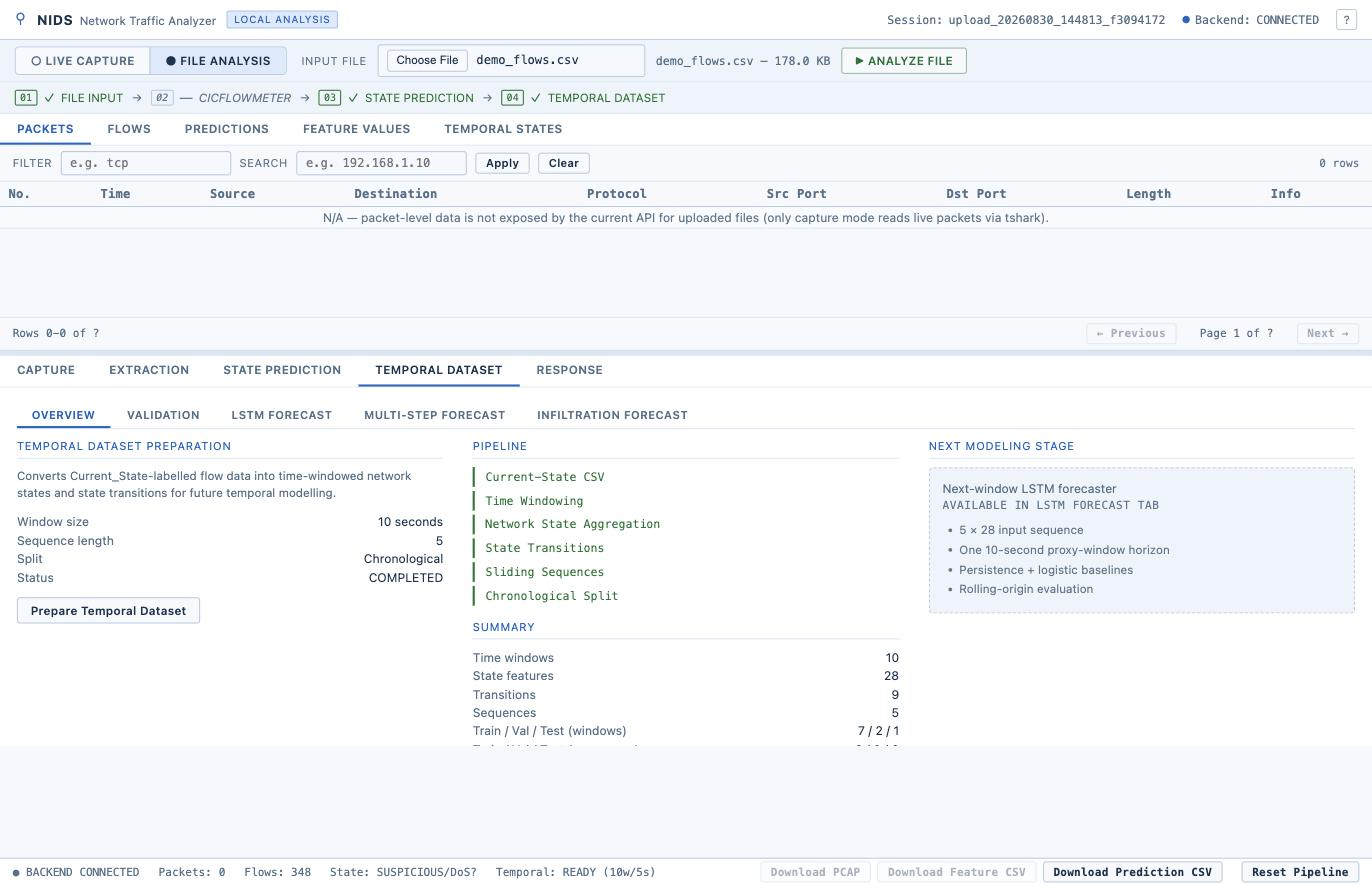
\includegraphics[width=\linewidth]{fig-temporal-overview.jpg}
\caption{The six-step temporal pipeline on the dashboard, with the run summary:
10 windows, 28 state features, 9 transitions, 5 sequences, a 7/2/1
window split. Short captures produce few windows --- the panel says so plainly
rather than padding.}
\end{figure}

\begin{figure}[H]\centering
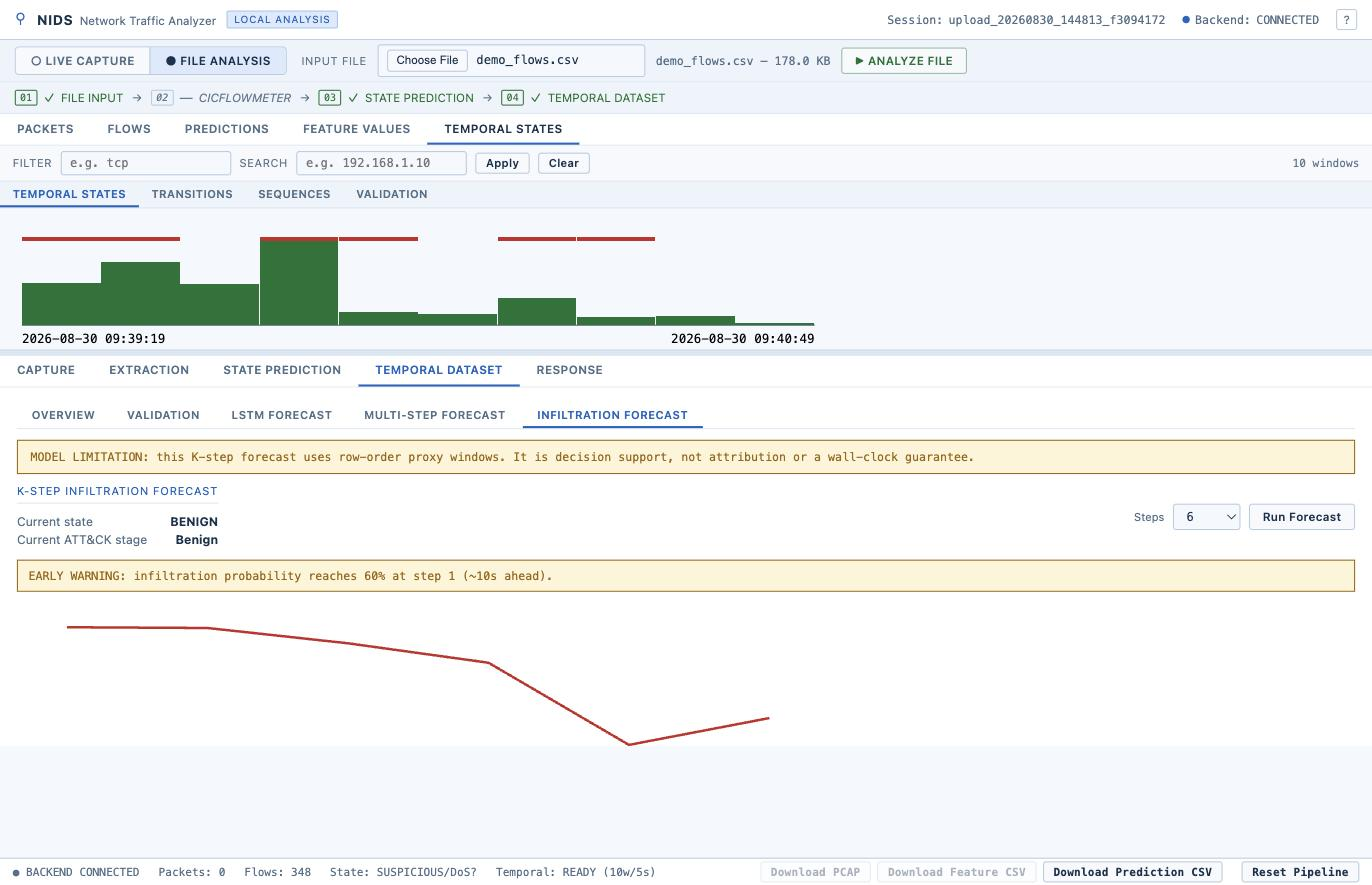
\includegraphics[width=\linewidth]{fig-temporal-states.jpg}
\caption{The windows over time. Bar height is flow count, colour is the dominant
class, a red tick marks a window with any attack flow. Timestamps are real
(here 09:39:19 to 09:40:49).}
\end{figure}

\subsection{Stage 4b --- The 10-check validation / leakage audit}
Before anyone trusts a forecast, \texttt{validate.py} re-checks a prepared
dataset read-only and reports each check PASS / WARNING / FAIL:

\begin{enumerate}[itemsep=1pt]
\item labels present and only the four known classes
\item timestamps parse, and are in order
\item exact-duplicate rows / duplicate IDs
\item missing / infinite cells
\item window duration exact, no overlaps, gaps flagged (expected)
\item all 28 features numeric, non-negative where the name implies it
\item transitions reference real windows and match the actual next state
\item sequence targets are exactly one window after the last input
\item the chronological split really is train $<$ val $<$ test in time
\item \textbf{leakage}: no sequence shared across splits, no window shared, the
  scaler saw training data only, no feature named like the target
\end{enumerate}

\begin{figure}[H]\centering
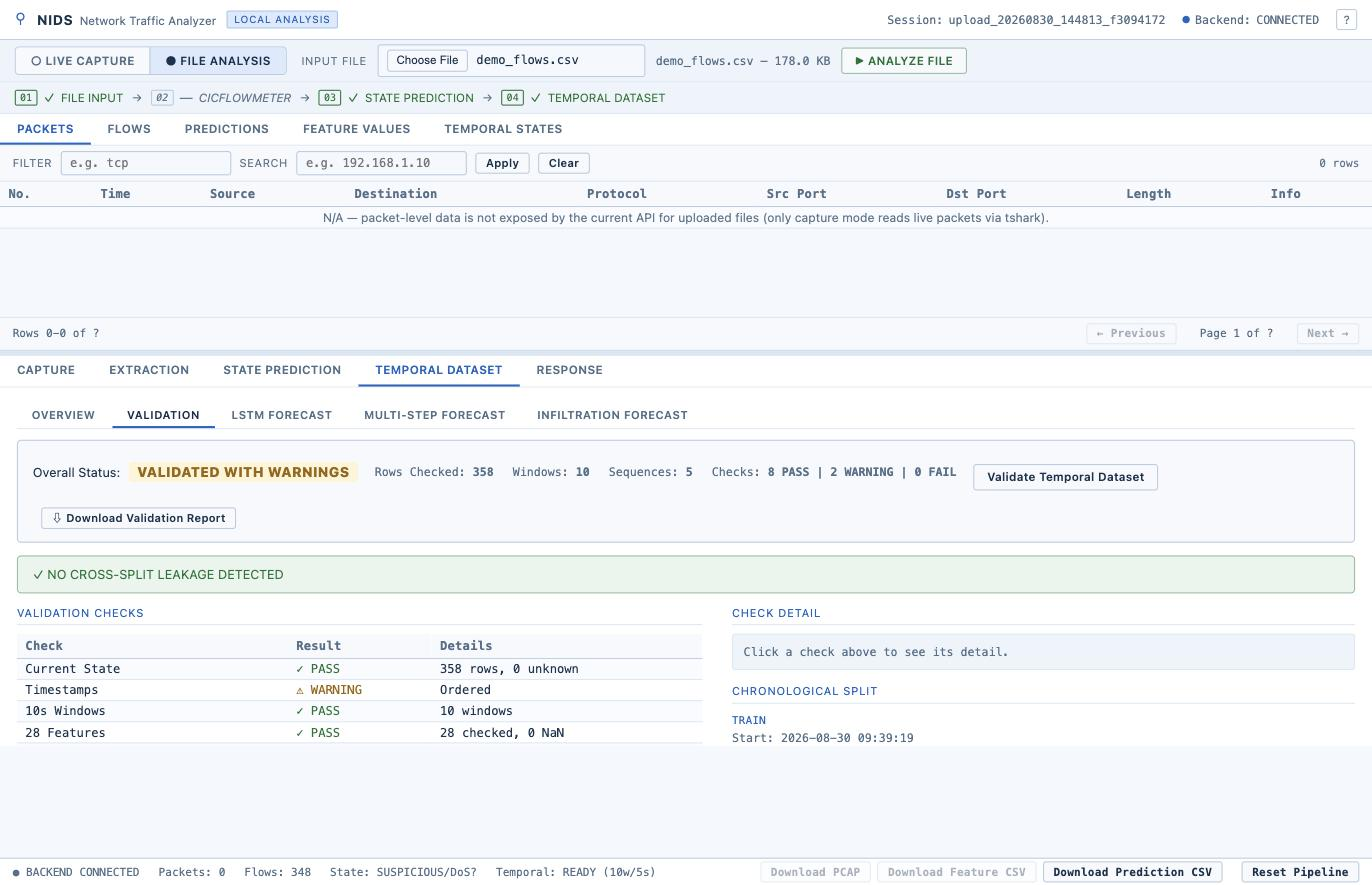
\includegraphics[width=\linewidth]{fig-validation.jpg}
\caption{A validation run: 8 PASS, 2 WARNING, 0 FAIL; ``NO CROSS-SPLIT LEAKAGE
DETECTED''. The Timestamps WARNING here is a benign ordering note, not a defect.}
\end{figure}

\section{Stage 5 --- Forecasting the next window (one-step LSTM)}

\subsection*{What it does, in plain words}
\begin{itemize}
\item Takes the last five 10-second windows and predicts the \emph{next}
  window's dominant state and an ``attack alert'' class, as probabilities.
\item The model is a small LSTM: 64 memory units, a shared 32-unit layer, then
  two 4-way softmax heads. Trained with a fixed random seed for reproducibility.
\item Trained on four CICIDS2017 weekday sessions. \textbf{Important honesty
  caveat:} one CSV row is treated as one ``proxy second'' and a window is
  10 \emph{rows}, so horizons are windows, not validated wall-clock seconds.
\item Model selection uses three expanding time-ordered folds; the winner is
  retrained; it is then scored on a strict final holdout against two baselines
  --- \emph{persistence} (predict the last state) and \emph{logistic
  regression}.
\item It is only ``activated'' (promoted to the live model) if it beats logistic
  regression on macro-F1 and DDoS recall and keeps the benign false-positive
  rate within one point. In practice DDoS is absent from the configured
  sessions, so the honest headline metric is the \emph{validation} split.
\end{itemize}

\begin{figure}[H]\centering
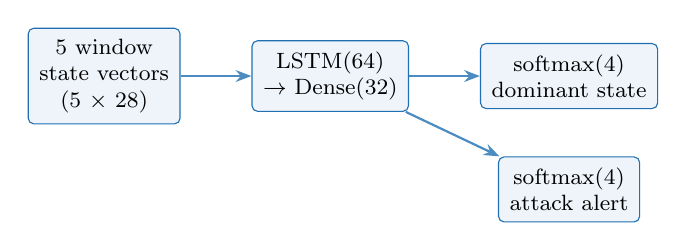
\begin{tikzpicture}[node distance=5mm and 9mm]
  \node[box] (h) {5 window\\state vectors\\(5 $\times$ 28)};
  \node[box,right=of h] (l) {LSTM(64)\\$\rightarrow$ Dense(32)};
  \node[box,right=of l] (d1) {softmax(4)\\dominant state};
  \node[box,below=6mm of d1] (d2) {softmax(4)\\attack alert};
  \draw[fl] (h)--(l); \draw[fl] (l)--(d1); \draw[fl] (l)--(d2);
\end{tikzpicture}
\caption{One-step forecaster (\texttt{backend/lstm/}). Two heads from one shared
body.}
\end{figure}

\begin{figure}[H]\centering
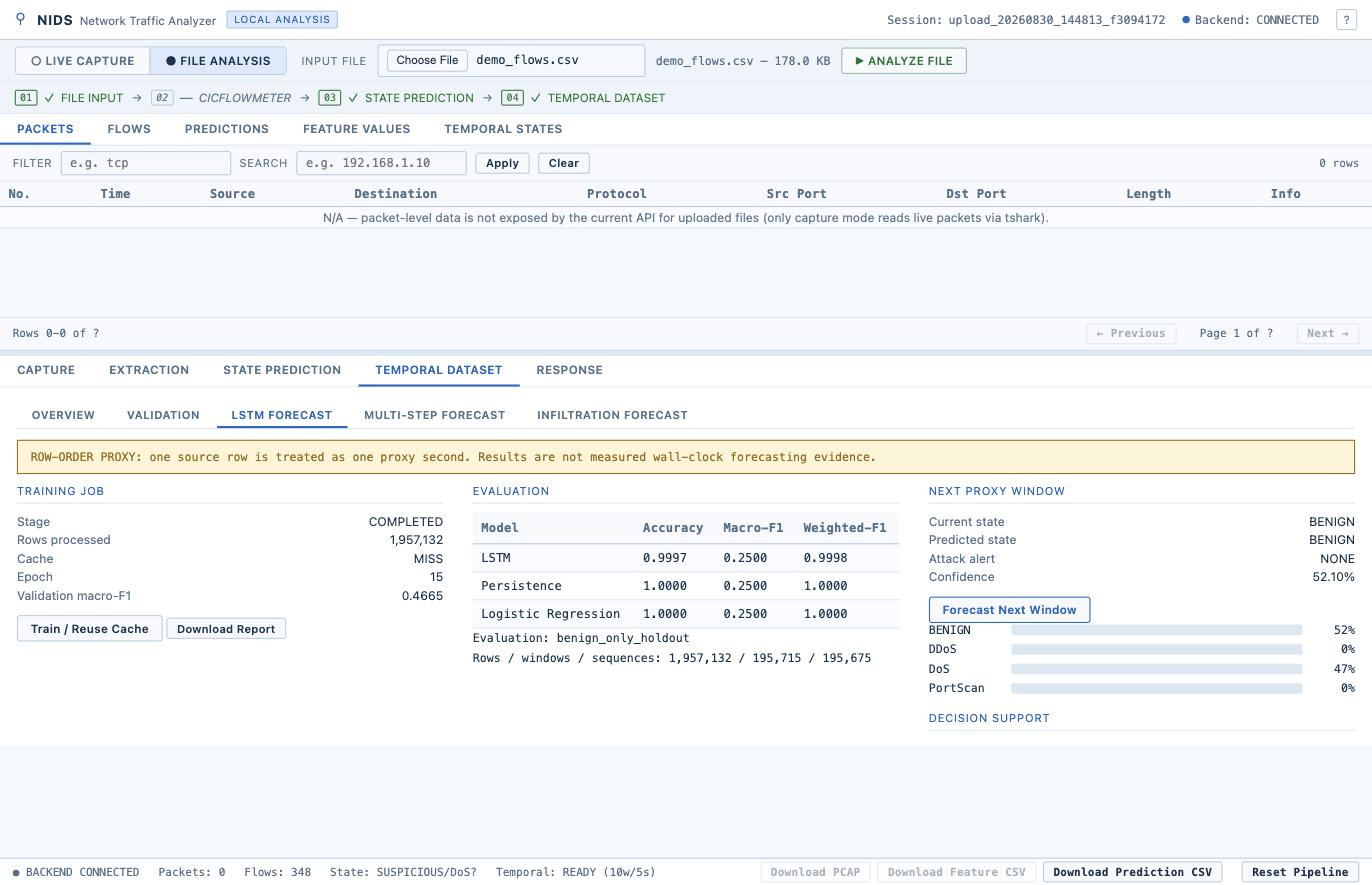
\includegraphics[width=\linewidth]{fig-lstm-forecast.jpg}
\caption{A live one-step forecast: current state BENIGN, predicted BENIGN,
attack alert NONE, confidence 52\%. The evaluation table compares the LSTM to
persistence and logistic-regression baselines; the row-order-proxy caveat is
shown at the top of the panel.}
\end{figure}

\subsection{Stage 5b --- The multi-step forecast (H1--H6)}
A second model (\texttt{backend/lstm\_multistep/}) predicts the next
\emph{six} windows in one shot (heads reshaped to $6\times4$). It adds:
\begin{itemize}
\item an \textbf{early-warning threshold} chosen to catch as many attacks as
  possible while keeping false alarms $\leq$5\%;
\item \textbf{onset / lead-time} metrics --- for cases where history is all
  benign and an attack really starts within six windows, how early or late the
  alarm fires;
\item a \textbf{degradation table} showing how accuracy falls off as the horizon
  grows.
\end{itemize}

\begin{figure}[H]\centering
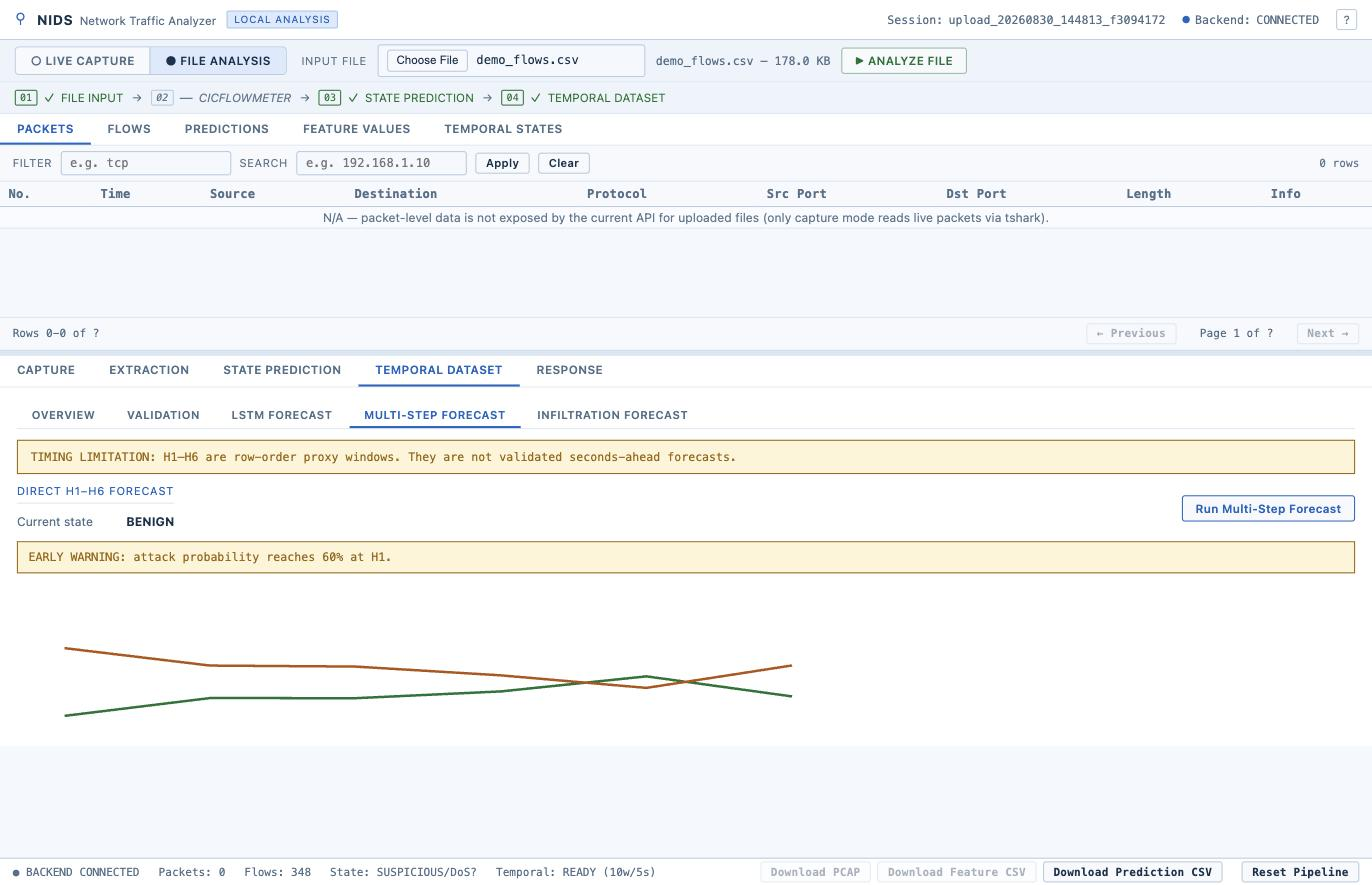
\includegraphics[width=\linewidth]{fig-multistep.jpg}
\caption{Multi-step: ``EARLY WARNING: attack probability reaches 60\% at H1'',
with the per-class probability trajectory across the six horizons.}
\end{figure}

\subsection{Stage 5c --- The infiltration forecast (world model)}
The world model (\texttt{backend/worldmodel/}) differs from the LSTMs by having
a \textbf{second, regression head that predicts the next window's full 28-number
state}. That means it can feed its own prediction back in and keep simulating
step after step --- an autoregressive ``rollout'' of K steps (default 6, max
24). It also exposes \textbf{attention weights} over the five input windows and
maps each predicted state to a kill-chain stage
(Recon\,$\to$\,\dots\,$\to$\,Impact).

\begin{figure}[H]\centering
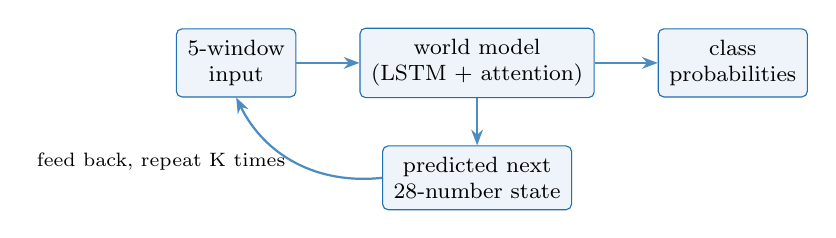
\begin{tikzpicture}[node distance=5mm and 8mm]
  \node[box] (seq) {5-window\\input};
  \node[box,right=of seq] (m) {world model\\(LSTM + attention)};
  \node[box,right=of m] (cls) {class\\probabilities};
  \node[box,below=6mm of m] (nxt) {predicted next\\28-number state};
  \draw[fl] (seq)--(m); \draw[fl] (m)--(cls); \draw[fl] (m)--(nxt);
  \draw[fl] (nxt.west) to[bend left=35] node[left,font=\scriptsize]{feed back, repeat K times} (seq.south);
\end{tikzpicture}
\caption{The rollout loop. Steps after the first are conditioned on the model's
own imagined states, not on real data --- hence ``forward-simulating world
model'' rather than ``one-step classifier''.}
\end{figure}

\begin{figure}[H]\centering
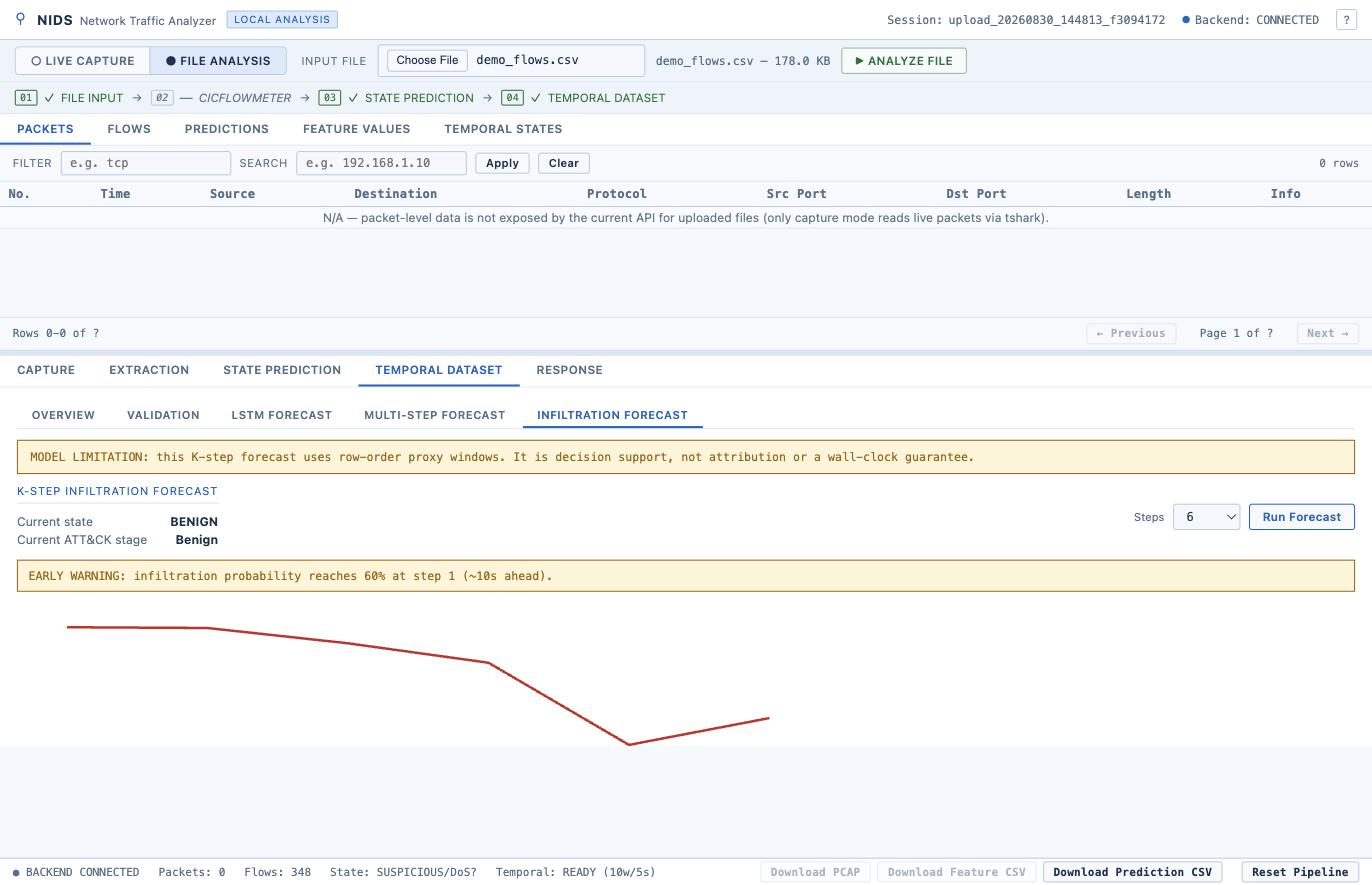
\includegraphics[width=\linewidth]{fig-infiltration.jpg}
\caption{Infiltration forecast: ``infiltration probability reaches 60\% at step
1 ($\sim$10\,s ahead)'', with the probability curve over the K steps and the
current ATT\&CK stage.}
\end{figure}

\section{Stage 6 --- MITRE ATT\&CK context}

The mapper (\texttt{mitre/mapper.py}) is deliberately restrained. It holds a
fixed table --- \texttt{PortScan}\,$\to$\,(T1595 Active Scanning, T1046 Network
Service Discovery); \texttt{DDoS}\,$\to$\,(T1498 and sub-techniques);
\texttt{DoS}\,$\to$\,(T1499) --- and, given the current state, the next-state
probabilities and the latest window's raw numbers, it produces technique
\emph{candidates} with:
\begin{itemize}
\item a \texttt{mapping\_status} of \texttt{POSSIBLE} or
  \texttt{INSUFFICIENT\_EVIDENCE};
\item a \texttt{mapping\_confidence} of 0.25, 0.55 or 0.65 --- explicitly typed
  \texttt{deterministic\_heuristic\_not\_calibrated};
\item human evidence sentences built from thresholds (port diversity, SYN
  volume, packet rate);
\item a severity (high / medium / informational), an operator playbook and an
  ``evidence needed'' list;
\item the offline ATT\&CK version (Enterprise v19.1), pinned and provenance-checked.
\end{itemize}
Every candidate carries the caveat that network-flow evidence alone cannot
confirm intent or host behaviour.

\begin{lstlisting}[caption={\texttt{nids mitre map --state PortScan --prob PortScan=0.7 --prob BENIGN=0.3} (abridged)}]
current_state: PortScan
predicted_next_state: PortScan
mapping_status: INSUFFICIENT_EVIDENCE
mitre_candidates:
  - technique_id: T1046   (Network Service Discovery, tactic Discovery)
    mapping_confidence: 0.25
    mapping_confidence_type: deterministic_heuristic_not_calibrated
    evidence: [ observed current network state is PortScan,
                LSTM next-state probability for PortScan is 0.700 ]
  - technique_id: T1595   (Active Scanning, tactic Reconnaissance)
    mapping_confidence: 0.25
attack_version: 19.1
severity: medium
\end{lstlisting}

\section{Stage 7 --- The dashboard, panel by panel}

\begin{table}[H]\centering\small
\begin{tabular}{@{}p{3.2cm}p{11.5cm}@{}}
\toprule
\textbf{Panel} & \textbf{What it shows} \\ \midrule
Live capture bar & interface picker, Start/Stop, duration + packet counters,
  packets-per-second sparkline, capture status dot. \\
File analysis bar & pick a \texttt{.pcap}/\texttt{.pcapng}/\texttt{.csv}, Analyze;
  offline, its own state machine. \\
Pipeline strip & four stages (Capture / CICFlowMeter / State prediction /
  Temporal), coloured by progress. \\
Packets / Flows / Predictions / Feature values / Temporal states & the left
  table, one tab each. \\
CAPTURE detail & every capture field, plus a hero block and (live) the sparkline. \\
EXTRACTION detail & input/output, flow and feature counts, the 77-feature list,
  and the ``compute packet-level features'' button. \\
STATE PREDICTION detail & the verdict hero, class distribution, signature hits,
  feature explanation, a flows-over-time timeline, and a classifier-metrics
  panel with a confusion matrix. \\
TEMPORAL DATASET detail & five inner tabs: Overview, Validation, LSTM forecast,
  Multi-step forecast, Infiltration forecast. \\
RESPONSE detail & the local response module (see below). \\
Status bar & backend state, packet/flow counters, the current verdict, temporal
  readiness, and export buttons. \\
\bottomrule
\end{tabular}
\caption{Dashboard map. Element IDs and the exact render function for each are
in Part~II.}
\end{table}

\begin{figure}[H]\centering
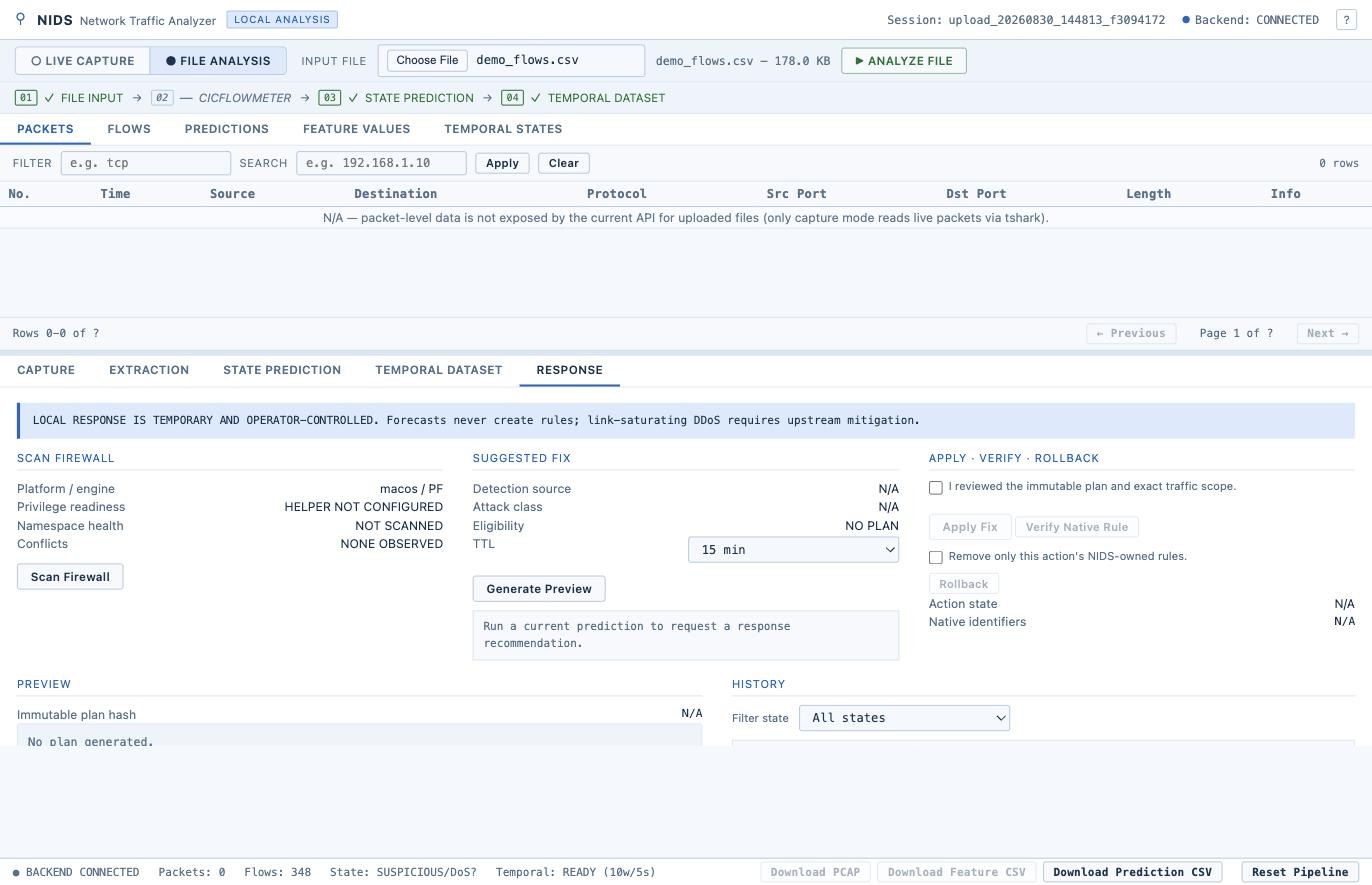
\includegraphics[width=\linewidth]{fig-response.jpg}
\caption{The RESPONSE panel --- an early active-response arm. It scans the local
firewall (here \texttt{macos / PF}), turns a detection into a \emph{suggested}
rule with a TTL, and gates apply / verify / rollback behind an explicit operator
checkbox. The banner is blunt: ``LOCAL RESPONSE IS TEMPORARY AND
OPERATOR-CONTROLLED. Forecasts never create rules; link-saturating DDoS requires
upstream mitigation.'' Protected addresses are allow-listed in
\texttt{config.json}.}
\end{figure}

\section{Stage 8 --- The command line}

Everything the dashboard does is also a \texttt{nids} subcommand (each is a thin
wrapper over the same service function the matching \texttt{/api/} route calls).

\begin{table}[H]\centering\small
\begin{tabular}{@{}p{4.2cm}p{10.5cm}@{}}
\toprule
\textbf{Command} & \textbf{Does} \\ \midrule
\texttt{serve} & run the API + dashboard on \texttt{:8765}. \\
\texttt{interfaces} & list capturable interfaces. \\
\texttt{capture start|packets|stat} & foreground capture; paginated packet read;
  \texttt{capinfos} of a pcap. \\
\texttt{extract <pcap>} & pcap $\rightarrow$ feature CSV. \\
\texttt{predict <csv>} & per-flow ANN prediction. \\
\texttt{predict-metrics} & precision/recall/F1/FPR + confusion matrix. \\
\texttt{explain --model ann|lstm|hgb <values.npy>} & submit a SHAP/attribution job. \\
\texttt{temporal prepare|validate} & build / audit a temporal dataset. \\
\texttt{lstm train|status|forecast|evaluate|report} & one-step forecaster. \\
\texttt{multistep dataset|train|evaluate|benchmark} & direct H1--H6. \\
\texttt{worldmodel train|status|forecast} & K-step infiltration forecaster. \\
\texttt{benchmark} & LSTM vs logistic-regression table. \\
\texttt{mitre map --state S --prob C=V} & ATT\&CK candidates for a forecast. \\
\texttt{pipeline show} & on-disk inventory of datasets, model versions, reports. \\
\bottomrule
\end{tabular}
\caption{The \texttt{nids} CLI. Exit codes: 0 ok, 2 usage, 3 missing
artifact/dataset, 4 runtime failure, 130 interrupted.}
\end{table}

\begin{lstlisting}[caption={\texttt{nids pipeline show} on the live repository}]
lstm_forecaster_versions: [ v1-3a5264a499ed, v1-6b89455037d9, v1-9f7373e0b3ad ]
lstm_forecaster_active: True
lstm_multistep_versions: [ v1-6d80927e0885 ]
worldmodel_trained: True
reports: { lstm_evaluation: True, multistep_evaluation: True, multistep_benchmark: True }
shap_backgrounds: { ann: True }
\end{lstlisting}

\begin{lstlisting}[caption={\texttt{nids benchmark} --- one-step LSTM vs logistic regression, validation split}]
model_version: v1-3a5264a499ed   headline_split: validation
                        LSTM        Logistic Regression
macro_f1                0.4623      0.4796
weighted_f1             0.9978      0.9988
attack_f1               0.8506      0.9191
attack_recall           0.9328      0.9076
attack_false_pos_rate   0.00188     0.00048
\end{lstlisting}

The LSTM's edge on this split is \emph{attack recall} (it misses fewer onsets),
not headline F1 --- on macro-F1 and false-positive rate the logistic baseline is
ahead. This is stated plainly in the evaluation report and is why activation
rarely fires.

\section{Project history}

\begin{table}[H]\centering\small
\begin{tabular}{@{}p{2.3cm}p{12.5cm}@{}}
\toprule
\textbf{Phase} & \textbf{What landed} \\ \midrule
Phase 0 & The original student project: a Keras ANN + scaler, three notebooks, a
  \texttt{tcpdump} wrapper. No backend, no automation --- and the prediction
  notebook never applied the scaler, so its committed output was the same four
  numbers for every row. This is the baseline the whole project fixed. \\
Phase 1 & Productisation: the end-to-end capture$\to$extract$\to$ANN pipeline, a
  FastAPI state machine, the dashboard, and Phase 3 LSTM forecasting +
  ATT\&CK context. \\
Phase 2 & Cross-platform capture (macOS friendly names, one-command setup) and
  the direct H1--H6 multi-step forecaster; a warnings clean-up. \\
Phase 3 & Explainability (gradient$\times$input), packet-level features, and the
  first product PDF; an ``honest overall state'' rework
  (dominant-class + attack ratio). \\
Phase 4 & Forecasting hardening, multi-interface capture, the logistic-regression
  benchmark, and a unified \texttt{nids} CLI + an async SHAP service. \\
Phase 5 & A run of honesty/robustness fixes: the status bar made to honour the
  confidence gate; cross-platform peak-RAM measurement; and the per-class
  percentage verdict gate (a minority class no longer triggers a red ``ATTACK''
  banner). The world model and its dashboard tab were added here. \\
\bottomrule
\end{tabular}
\caption{From a broken single notebook to an offline capture$\to$forecast
pipeline with a CLI, a SHAP service and a restrained ATT\&CK layer.}
\end{table}

\clearpage
\part*{Part II --- Function index}
\addcontentsline{toc}{section}{PART II --- Function index}

Every public function and class, grouped by file, one line each. Use this to
find the exact place a behaviour lives.

\newcommand{\fnrow}[3]{\texttt{#1} & \texttt{#2} & #3 \\}
\newenvironment{fntable}[1]{%
  \subsection*{#1}
  \begin{longtable}{@{}p{4.4cm}p{2.7cm}p{7.2cm}@{}}
  \toprule \textbf{Name} & \textbf{Location} & \textbf{What it does} \\ \midrule
  \endfirsthead
  \toprule \textbf{Name} & \textbf{Location} & \textbf{What it does} \\ \midrule
  \endhead
  \bottomrule \endfoot
}{\end{longtable}}

\begin{fntable}{backend/capture/capture.py}
\fnrow{list\_interfaces}{c.py:180}{list real capturable NICs (dumpcap/tcpdump -D), friendly names on macOS.}
\fnrow{start\_capture}{c.py:518}{build and launch the dumpcap/tcpdump command line; 0.5\,s sanity wait.}
\fnrow{stop\_capture}{c.py:760}{user stop; SIGINT then escalate; safe if already exited.}
\fnrow{check\_and\_finalize}{c.py:799}{on every poll: detect self-exit / duration / 600\,s safety, finalize.}
\fnrow{\_finalize}{c.py:703}{shared stop tail: stamp end time, parse drops, read real packet count.}
\fnrow{read\_packets}{c.py:444}{paginated per-packet rows via a tshark frame-range filter.}
\fnrow{\_capfile\_stats}{c.py:360}{ask capinfos for real packet count + duration.}
\fnrow{validate\_and\_stat\_pcap}{c.py:393}{strict pcap check for uploads (raises on 0 packets).}
\fnrow{\_parse\_capture\_drops}{c.py:673}{pull received/dropped counts from the tool's exit summary.}
\fnrow{CaptureSession}{c.py:260}{dataclass: process handle, path, targets, results, stderr tail.}
\end{fntable}

\begin{fntable}{backend/extraction/}
\fnrow{run\_extraction}{extract.py:28}{replay a pcap through CICFlowMeter once -> one feature CSV.}
\fnrow{run\_parallel\_extraction}{parallel\_extract.py:69}{split big pcaps with editcap, extract chunks in parallel, concat.}
\fnrow{extract\_packet\_features}{packet\_features.py:47}{per-flow TTL / TCP-window / retransmission / fragment / payload stats (Scapy).}
\fnrow{port\_scan\_signature}{packet\_features.py:142}{record the order dst ports were first contacted; classify the sweep.}
\fnrow{\_classify\_port\_order}{packet\_features.py:198}{sequential / strided / randomised / none.}
\fnrow{packet\_features\_summary}{packet\_features.py:216}{JSON bundle for the PACKET FEATURES panel.}
\end{fntable}

\begin{fntable}{backend/prediction/features.py}
\fnrow{TRAINING\_FEATURES}{features.py:25}{the ordered list of 77 feature-column names (do not reorder).}
\fnrow{match\_columns}{features.py:105}{map any CSV's columns to the 77 by canonical token signature; raises on a miss.}
\fnrow{\_canonical\_signature}{features.py:95}{reduce a column name to a sorted tuple of canonical tokens.}
\fnrow{is\_id\_or\_label\_column}{features.py:136}{true for identifier/label columns (never features).}
\end{fntable}

\begin{fntable}{backend/prediction/predict.py}
\fnrow{predict\_csv}{predict.py:250}{main: read CSV, score every flow, run signatures, write labels back, return the result dict.}
\fnrow{summarize\_states}{predict.py:72}{per-class counts -> headline verdict + confidence, applying the 20\% gate.}
\fnrow{\_load\_artifacts}{predict.py:216}{load ISAA\_ANN.h5 + minmax.bin once (cached).}
\fnrow{\_flow\_feature\_values}{predict.py:159}{per row: 21 curated feature values + a TCP-flag bitmask.}
\fnrow{CLASS\_NAMES}{predict.py:43}{[BENIGN, DDoS, DoS, PortScan] --- softmax index order.}
\fnrow{MIN\_ATTACK\_RATIO\_x}{predict.py:68}{verdict-gate thresholds, read from config/config.json.}
\end{fntable}

\begin{fntable}{backend/prediction/signatures.py}
\fnrow{flow\_signatures}{signatures.py:66}{whole-table rule layer: rolling flood, SYN flood, port sweep -> per-row states + summary.}
\fnrow{\_port\_access\_pattern}{signatures.py:49}{classify how a set of dst ports was walked.}
\fnrow{DDOS/DOS/PORTSCAN\_x}{signatures.py:29}{the rule thresholds (fan-in 20, pkts/s 100, SYN 20, ACK-ratio 0.2, ports 20, bytes 400).}
\end{fntable}

\begin{fntable}{backend/prediction/ (explain, SHAP, challenger, metrics)}
\fnrow{attribute}{explain.py:29}{gradient x input saliency for the ANN (one backward pass).}
\fnrow{driving\_features}{explain.py:74}{capture-wide top 10 features by mean absolute contribution.}
\fnrow{tree\_explanation / gradient\_explanation}{shap\_service.py:56/76}{real SHAP for the tree challenger / a Keras model.}
\fnrow{gradient\_input\_fallback}{shap\_service.py:99}{used when real SHAP throws; is\_shap:false.}
\fnrow{ExplanationJobs.submit}{shap\_service.py:137}{async attribution job store (thread pool, cache by hash).}
\fnrow{submit\_explanation}{explanation\_runtime.py:33}{wire a model kind to the right explainer; needs a background .npy.}
\fnrow{fit\_challenger / train\_flow\_challenger}{flow\_challenger.py:32/66}{HistGradientBoosting alternative model (not auto-promoted).}
\fnrow{evaluate\_ann\_metrics}{metrics.py:167}{real CICIDS2017 ground-truth metrics, or None.}
\fnrow{proxy\_agreement\_metrics}{metrics.py:231}{fallback: ANN-vs-signature agreement (not ground truth).}
\fnrow{compute\_metrics}{metrics.py:136}{precision/recall/F1/support, macro/weighted F1, confusion matrix.}
\end{fntable}

\begin{fntable}{backend/temporal/}
\fnrow{prepare\_temporal\_dataset}{temporal\_dataset.py:81}{orchestrator: CSV -> windows -> states -> sequences -> split -> files.}
\fnrow{parse\_timestamps}{windowing.py:31}{read the time column, tracking unparseable rows honestly.}
\fnrow{assign\_windows}{windowing.py:77}{label each flow with its 10-second slot.}
\fnrow{build\_temporal\_states}{state\_builder.py:20}{per window: 28-number state vector + dominant class + attack\_present.}
\fnrow{build\_state\_transitions}{sequence\_builder.py:19}{window -> next-window pairs with real time delta.}
\fnrow{build\_sequences}{sequence\_builder.py:55}{slide 5 windows in, 1 out; strictly chronological.}
\fnrow{chronological\_split}{splitting.py:22}{first 70\% / next 15\% / last 15\% by time.}
\fnrow{fit\_scaler\_on\_train}{splitting.py:51}{MinMaxScaler on training windows only.}
\fnrow{run\_all\_checks}{validation.py:73}{the 7 build-time gate checks.}
\fnrow{validate\_temporal\_dataset}{validate.py:544}{the 10-check read-only audit incl. O(n) leakage detection.}
\fnrow{STATE\_FEATURE\_NAMES}{schema.py:72}{the 28-element state-vector schema.}
\end{fntable}

\begin{fntable}{backend/lstm/ (one-step forecaster)}
\fnrow{train\_forecaster}{training.py:283}{full run: windows -> 3-fold selection x 3 loss recipes -> retrain -> holdout vs baselines -> report.}
\fnrow{build\_model}{training.py:83}{LSTM(64)->Dropout(0.3)->Dense(32)-> two softmax(4) heads.}
\fnrow{forecast\_latest}{training.py:547}{run the active model on the recent 5 windows -> next-window probabilities + MITRE map.}
\fnrow{\_load\_recent\_windows}{training.py:495}{last 5 contiguous prepared windows to forecast from (shared by all three forecasters).}
\fnrow{rolling\_origin\_windows}{training.py:103}{3 expanding time-ordered folds for model selection.}
\fnrow{\_persistence / \_logistic}{training.py:229/238}{the two baselines on the holdout.}
\fnrow{evaluate\_predictions}{evaluation.py:111}{the metric battery: 4-class macro-F1 and binary attack-vs-benign.}
\fnrow{cicids\_ground\_truth\_state}{dataset.py:35}{map a CICIDS2017 Label to BENIGN/DDoS/DoS/PortScan or None.}
\fnrow{prepare\_session\_windows}{dataset.py:275}{build (or cache) proxy windows for one CICIDS2017 session (10 rows = 1 window).}
\fnrow{evaluate\_saved\_artifact}{rigorous\_evaluation.py:442}{honest re-evaluation + 8-check leakage audit; writes the report.}
\fnrow{start\_training}{jobs.py:56}{spawn the training process; status file polled by the UI.}
\end{fntable}

\begin{fntable}{backend/lstm\_multistep/ (direct H1--H6)}
\fnrow{train\_multistep}{training.py:206}{build dataset -> train the 6x4-head model -> threshold selection -> per-horizon eval -> activation gate.}
\fnrow{build\_model}{training.py:50}{LSTM(64)->Dense(32)-> Dense(24)->Reshape(6,4)->softmax, twice.}
\fnrow{forecast\_latest}{training.py:304}{one forward pass -> 6 horizons; earliest horizon whose attack prob >= threshold.}
\fnrow{build\_multistep\_sequences}{dataset.py:24}{slide 5 history + 6 target windows.}
\fnrow{split\_session\_windows}{dataset.py:82}{5 train sessions, 2 validation, Friday-DDoS cut 60/20/20 with embargo.}
\fnrow{select\_early\_warning\_threshold}{evaluation.py:22}{pick the alarm cutoff: max attack-F1 s.t. FPR <= 5\%.}
\fnrow{onset\_metrics}{evaluation.py:41}{early / on-time / late detection and mean lead windows.}
\fnrow{degradation\_table}{evaluation.py:70}{how accuracy/F1 decay from H1 to H6.}
\end{fntable}

\begin{fntable}{backend/worldmodel/ (K-step infiltration)}
\fnrow{build\_world\_model}{model.py:26}{LSTM(64, return\_sequences) + attention over 5 steps + two heads: class softmax(4) and next-state Dense(28).}
\fnrow{rollout}{model.py:52}{predict next state + feature vector, slide it onto the input, repeat K times.}
\fnrow{train\_world\_model}{training.py:138}{build 5->1 pairs with a 28-d regression target; loss weights 1.0 / 0.3; macro-F1 >= 0.40 => VALIDATED.}
\fnrow{forecast}{engine.py:102}{roll K steps -> per-step infiltration probability, risk level, kill-chain stage, top features, attended windows.}
\fnrow{\_feature\_attribution}{engine.py:74}{gradient x input over the 28 state features for the "not benign" score.}
\fnrow{state\_to\_stage / presentation\_state}{killchain.py:40/44}{4-class state -> kill-chain rung + tactic id + ladder.}
\fnrow{risk\_level}{killchain.py:64}{>=0.80 high, >=0.50 medium, else low.}
\end{fntable}

\begin{fntable}{backend/mitre/mapper.py}
\fnrow{map\_forecast}{mapper.py:172}{state + probabilities + features -> technique candidates + severity + playbook.}
\fnrow{\_behavior\_evidence}{mapper.py:99}{turn raw window numbers into human evidence sentences (fixed thresholds).}
\fnrow{\_guidance}{mapper.py:138}{fixed playbooks per state (DDoS/DoS high, PortScan medium, else informational).}
\fnrow{AttackMetadataStore.load}{mapper.py:33}{read + strictly validate the offline ATT\&CK v19.1 subset.}
\fnrow{STATE\_TECHNIQUES}{mapper.py:76}{PortScan->(T1595,T1046); DDoS->(T1498,.001,.002); DoS->(T1499).}
\end{fntable}

\begin{fntable}{backend/api/main.py (endpoints)}
\fnrow{GET /api/pipeline}{main.py:377}{the whole capture->predict snapshot.}
\fnrow{POST /api/capture/start|stop}{main.py:145/170}{start / stop a live capture.}
\fnrow{GET /api/capture/status|packets}{main.py:212/219}{live status; paginated packet page.}
\fnrow{POST /api/extract|predict}{main.py:252/326}{background extraction / prediction jobs.}
\fnrow{GET /api/predict/metrics}{main.py:342}{ground-truth or proxy classifier metrics.}
\fnrow{POST /api/upload}{main.py:410}{offline file analysis (pcap or csv), own state machine.}
\fnrow{POST /api/temporal/prepare|validate}{main.py:519/640}{build / audit a temporal dataset.}
\fnrow{POST /api/lstm/forecast|.../multistep}{main.py:785/793}{one-step / H1--H6 forecast.}
\fnrow{POST /api/worldmodel/forecast}{main.py:818}{K-step infiltration forecast.}
\fnrow{GET /api/benchmark}{main.py:833}{LSTM vs logistic-regression table.}
\end{fntable}

\begin{fntable}{frontend/app.js (render functions, grouped)}
\fnrow{predVerdict}{app.js:1138}{shared display verdict: none / benign / suspicious / attack from confidence.}
\fnrow{renderPredictionTab}{app.js:1148}{the verdict hero, dominant/alert sub-line, flagged-flows line, sub-panels.}
\fnrow{renderClassDistribution}{app.js:1422}{per-class bar with count and \% of flows.}
\fnrow{renderSignatureHits}{app.js:1220}{one row per fired signature rule.}
\fnrow{renderDrivingFeatures}{app.js:1239}{SHAP job result if present, else gradient x input; signed bars.}
\fnrow{renderClassifierMetrics}{app.js:1091}{ground-truth vs proxy badge, per-class table, confusion heat-map.}
\fnrow{renderPredictionFlowsTimeline}{app.js:1350}{benign/attack flows per minute + mean confidence line (inline SVG).}
\fnrow{renderTemporalTab / renderValidationTab}{app.js:1439/1661}{the 6-step strip + summary; the 10-check grid + leakage banner.}
\fnrow{renderLstmTab}{app.js:1492}{training job rows, evaluation table, next-window probabilities, MITRE decision support.}
\fnrow{renderMultistepTab / renderWorldModelTab}{app.js:1548/1594}{early-warning banner + trajectory chart + per-horizon / per-step details.}
\fnrow{renderCaptureTab / renderCaptureRateSparkline}{app.js:887/1401}{capture fields + hero; client-side packets/sec sparkline.}
\fnrow{startPolling / refreshPipeline}{app.js:347/313}{the 1.2\,s master poll of /api/pipeline.}
\end{fntable}

\clearpage
\part*{Part III --- Attacks, and how this app handles them}
\addcontentsline{toc}{section}{PART III --- Attacks and how this app handles them}

\section{The three levers}

\begin{table}[H]\centering\small
\begin{tabular}{@{}p{2.3cm}p{7.3cm}p{4.7cm}@{}}
\toprule
\textbf{Lever} & \textbf{App machinery} & \textbf{Output} \\ \midrule
\textbf{FLAG} & 77 flow features -> ANN; the signature layer;
  packet-level features; the verdict gate; the MITRE mapper; SHAP. &
  per-flow label, capture verdict, ATT\&CK technique, ``why''. \\
\textbf{PREDICT} & 10-second windows -> one-step LSTM + direct H1--H6
  + world-model rollout; early-warning threshold; onset/lead-time. &
  ``class X likely in +N windows'', infiltration curve, earliest-alarm step. \\
\textbf{PREVENT} & the response ladder keyed off verdict + forecast:
  protected-address allow-list -> rate-limit -> eBPF/XDP
  drop -> firewall rule -> quarantine VLAN -> host isolate; human-in-loop
  above rate-limit; auto-rollback; audit. &
  contained blast radius, recommended hardening. \\
\bottomrule
\end{tabular}
\end{table}

Effort tags below: \textbf{[now]} works today; \textbf{[+sig]} one signature
rule; \textbf{[+feat]} one feature/parser; \textbf{[+model]} a new model head or
module; \textbf{[+int]} an enterprise integration (firewall / NAC / EDR / AD /
WAF / DNS-RPZ).

\section{Attack-by-attack}

\newcommand{\atk}[4]{%
\subsection*{#1}
\begin{tabular}{@{}p{1.9cm}p{13cm}@{}}
\textbf{Flag} & #2 \\[2pt]
\textbf{Predict} & #3 \\[2pt]
\textbf{Prevent} & #4 \\
\end{tabular}}

\atk{DoS (single-source: SYN/ACK/RST flood, slowloris, slow-read, connection exhaustion)}
{\textbf{[now]} ANN \texttt{DoS} class + the \texttt{syn-flood} signature (SYN >= 20, ACK/SYN <= 0.2, >= 100 pkts/s); packet-rate + half-open ratio. Slowloris \textbf{[+sig]}: count of long idle half-open connections.}
{\textbf{[now]} world-model rollout on packet-rate + SYN-ratio slope -> infiltration curve; earliest-alarm step at threshold 0.60.}
{\textbf{[+int]} rate-limit -> eBPF/XDP drop of the source; recommend SYN cookies and connection timeouts.}

\atk{DDoS (volumetric L3/4, amplification/reflection, L7 HTTP flood, pulse-wave)}
{\textbf{[now]} ANN \texttt{DDoS} + the \texttt{rolling-source-fanin-flood} signature; source-IP entropy. Reflection \textbf{[+sig]}: response-without-request + amplification ratio by port (53/123/11211/1900/389).}
{\textbf{[now]} fan-in ramp + per-victim flow-ratio trend feed H1--H6; \textbf{[+int]} edge/NetFlow sensors see the ramp minutes before saturation.}
{\textbf{[+int]} BGP blackhole / Flowspec / upstream scrubbing; XDP drop by source prefix; WAF rate rules + JS challenge for L7.}

\atk{Phishing (spearphish link/attachment, credential-harvest site, BEC)}
{\textbf{[+feat]} DNS to newly-registered / typosquat / punycode domains; TLS SNI + certificate age/issuer for look-alike sites; \textbf{[+int]} mail-gateway logs. Post-click: \textbf{[now]} the callback flow after the payload runs is caught by the signature + ANN.}
{\textbf{[+model]} ``recon domain resolved but not yet contacted'' watch-list; a fleet-wide spike in look-alike DNS = campaign early warning.}
{\textbf{[+int]} DNS-RPZ sinkhole the domain; block egress to the IP; force a password reset via the AD API; push the IOC to the mail gateway.}

\atk{Man-in-the-middle (ARP spoof, LLMNR/NBNS poisoning, rogue DHCP, DNS spoof, SSL strip, rogue AP, BGP hijack)}
{\textbf{[+feat]} IP-to-MAC binding churn, gratuitous-ARP rate, duplicate IP; rogue DHCP = unexpected OFFER source; DNS response anomaly / DNSSEC-fail; HTTP where HTTPS was expected (SSL strip). Rogue AP needs \textbf{[+int]} WIPS.}
{ARP-storm precursor before poisoning completes; BGP: origin-AS change against an RPKI baseline.}
{\textbf{[+int]} trigger Dynamic ARP Inspection / DHCP snooping / port-security via NAC; quarantine the port/MAC to an isolation VLAN.}

\atk{Port scanning / reconnaissance (SYN/FIN/NULL/Xmas/UDP scan, slow scan, distributed scan, OS/version fingerprint, vuln scan)}
{\textbf{[now]} the \texttt{port-sweep} signature (>= 20 distinct dst ports, mean fwd bytes <= 400) + the packet-order classifier; ANN \texttt{PortScan}.}
{\textbf{[now]} \emph{the single best leading indicator} --- scan then exploit. Scan intensity + target spread feed the forecaster; the world model raises ``exploit likely at host X in +N windows''.}
{\textbf{[+int]} tarpit / rate-limit / block the scanner prefix; move the probed host behind a stricter ACL; \textbf{[track H]} redirect to a honeypot for a clean label.}

\atk{Brute force / credential attacks (SSH/RDP/SMB/HTTP-auth brute force, password spraying, credential stuffing, Kerberoasting)}
{\textbf{[+feat]} a failed-auth graph (source IP x account x service), velocity + failure ratio; \textbf{[+int]} AD / auth-log fusion for spraying (1 try, many accounts) and Kerberoasting (rare SPN TGS requests).}
{a distributed low-and-slow login ramp across the fleet -> ``account-takeover attempt in progress''.}
{\textbf{[+int]} block the source, enforce MFA / lockout, disable the targeted account, impossible-travel rule.}

\atk{Malware C2 / botnet (HTTP/HTTPS beaconing, DNS C2, Cobalt Strike / Sliver, fast-flux, DGA domains)}
{\textbf{[+feat]} a beacon detector = interval + jitter clustering on periodic small egress; JA3/JA4 + malleable-profile fingerprint; DGA = query-name entropy + length + NXDOMAIN rate. \textbf{[now]} the loud ones are already caught.}
{a new periodic egress edge emerging after compromise = ``host X is now controlled''; feeds the world model -> forecast lateral movement next.}
{\textbf{[+int]} egress allow-list, DNS sinkhole the C2, XDP drop the IP, isolate the host via EDR; push the IOC fleet-wide.}

\atk{Lateral movement (SMB / PsExec / WMI / WinRM / RDP, pass-the-hash, SMB relay)}
{\textbf{[+model, track C]} the communication-graph GNN --- new east-west host-pair edges, unusual service use, anomalous paths; \textbf{[+feat]} admin-share access outside the baseline.}
{\textbf{[track C]} the first anomalous east-west edge -> forecast the next hops (graph link-prediction). This is the ``Campaign'' view.}
{\textbf{[+int]} micro-segmentation rule push, quarantine both endpoints, kill the SMB session, disable the credential.}

\atk{Data exfiltration (bulk HTTPS upload, DNS tunnelling, ICMP tunnelling, cloud-storage exfil, low-and-slow)}
{\textbf{[+feat]} upload/download byte asymmetry per host; DNS query volume + entropy + TXT/NULL record rate; ICMP payload size/entropy; destination novelty (never-seen ASN/domain).}
{\textbf{[+model]} internal ``staging'' (large internal reads / share enumeration) precedes egress by minutes--hours -> warn before data leaves.}
{\textbf{[+int]} egress byte-cap, block the destination, DNS-RPZ, DLP / CASB trigger, isolate the host.}

\atk{Ransomware (delivery -> C2 -> lateral spread -> share enumeration -> mass encryption over SMB)}
{\textbf{[+feat]} SMB file-op rate + read-then-write-rename burst on shares; internal SMB fan-out; a workstation contacting the backup server; \textbf{[track H]} a canary-file touch = instant high confidence.}
{\textbf{[track C+E]} the lateral phase (often hours) is the warning window --- graph anomaly + forecast ``encryption imminent on segment Y''.}
{\textbf{[+int]} isolate the host (EDR), block SMB between segments, disable the spreading account, snapshot/lock backups.}

\atk{Web application attacks (SQLi, XSS, RCE, LFI/RFI, path traversal, SSRF, XXE)}
{\textbf{[+feat]} a char-level model on request strings from cleartext HTTP or \textbf{[+int]} WAF-mirrored logs; payload signatures; SSRF = the app server suddenly talks to internal / metadata IPs.}
{a recon 404-scan / parameter-fuzz burst precedes the working exploit.}
{\textbf{[+int]} push a WAF block rule, block the source, rate-limit the endpoint.}

\atk{DNS attacks (cache poisoning, hijack, tunnelling, DGA, NXDOMAIN flood, subdomain enumeration)}
{\textbf{[+feat]} a DNS parser: response anomaly / DNSSEC-fail (poisoning); query entropy + NXDOMAIN rate (DGA/tunnel); rapid unique-subdomain rate (enumeration).}
{a DGA burst = malware present but pre-C2 -> warn before the successful callback.}
{\textbf{[+int]} RPZ sinkhole, force resolver DNSSEC validation, block the client.}

\atk{Spoofing (IP / MAC / email)}
{\textbf{[+feat]} IP spoof = TTL / OS-fingerprint vs the claimed source, RFC2827 ingress violation; MAC spoof = OUI vs behaviour; email via \textbf{[+int]} SPF/DKIM/DMARC in mail logs.}
{spoofed-source recon usually precedes a reflection DDoS or a session attack.}
{\textbf{[+int]} uRPF / BCP38 filter push, port-security, drop at the edge.}

\atk{VPN / remote-access attacks (VPN brute force, appliance-CVE exploit, session hijack)}
{\textbf{[+feat]} auth-failure rate on the concentrator; post-auth behaviour that doesn't match the user baseline; exploit = a malformed handshake / unexpected admin path.}
{brute-force ramp -> successful login -> immediate internal scan = takeover in progress.}
{\textbf{[+int]} block the source, force MFA re-auth, kill the tunnel, apply the CVE patch advisory.}

\atk{Wireless attacks (deauth flood, evil twin, WPA handshake capture, KRACK)}
{\textbf{[+int]} needs a WIPS feed --- deauth-frame rate, duplicate BSSID/SSID, rogue-AP MAC.}
{---}
{\textbf{[+int]} WIPS containment, 802.1X + PMF, rogue-AP switchport shutdown.}

\atk{IoT / OT attacks (Mirai-style recruitment via telnet/23, Modbus/DNP3 unauthorised write, OT protocol scan)}
{\textbf{[+feat]} a protocol-aware parser + a command allow-list model; a telnet/23 spike; unexpected function codes / write-coil operations.}
{an OT read-burst / enumeration precedes a write attack.}
{\textbf{[+int]} OT-DMZ rule, unidirectional-gateway recommendation, block the source, allow-list commands.}

\atk{Insider threat}
{\textbf{[+model]} a per-user / per-host behaviour baseline --- off-hours bulk transfer, access to systems outside the user's role, mass download.}
{an escalating access-scope trend before the big exfil.}
{\textbf{[+int]} alert + step-up auth + revoke access; DLP hold.}

\atk{Supply-chain / third-party}
{\textbf{[+feat]} egress to a new update / CI endpoint; a build server talking to the internet unexpectedly; a vendor-VPN source doing internal recon.}
{anomalous build-infra egress before the payload spreads.}
{\textbf{[+int]} egress allow-list for build infra, isolate the vendor segment, SBOM + signed-artifact check.}

\atk{TLS/SSL attacks (downgrade, strip, weak cipher, certificate abuse, JA3 mismatch)}
{\textbf{[+feat]} a TLS parser --- version/cipher downgrade, a self-signed / short-lived certificate to a sensitive destination, a client JA3 that doesn't match the claimed app.}
{---}
{\textbf{[+int]} block the connection, enforce a minimum-TLS policy, alert on certificate anomalies.}

\atk{Cryptojacking}
{\textbf{[+feat]} a Stratum-protocol fingerprint / known mining-pool IP+port; steady long-lived low-bandwidth egress with a mining JA3.}
{a new host joining a pool = a compromise indicator.}
{\textbf{[+int]} block pool egress, isolate the host.}

\atk{Living-off-the-land (certutil / bitsadmin download, PowerShell remoting, WMI exec)}
{\textbf{[+feat]} a user-agent + destination pattern for LOLBin downloads; WinRM/5985 from non-admin hosts; correlate with \textbf{[+int]} EDR process telemetry.}
{the first LOLBin download -> forecast lateral movement / C2 next.}
{\textbf{[+int]} block the download URL, isolate the host, disable WinRM on the segment.}

\atk{Evasion / protocol abuse (fragmentation, TTL games, domain fronting, packet padding, timing evasion)}
{\textbf{[+feat]} a fragment-overlap / tiny-fragment detector; SNI $\neq$ Host (fronting); \textbf{[B track]} a packet size/timing sequence model is padding-resistant.}
{---}
{\textbf{[+int]} reassemble-then-inspect, block fronting CDNs by policy, drop overlapping fragments.}

\atk{Zero-day / novel exploit}
{\textbf{[+model, D track]} a self-supervised anomaly model trained on benign traffic --- scores ``never seen this behaviour''; no signature needed.}
{an anomaly cluster forming across hosts = a campaign, even without a label.}
{\textbf{[+int]} quarantine the anomalous segment, capture full PCAP for IR, human triage.}

\section{Coverage --- an honest table}

\begin{table}[H]\centering\small
\begin{tabular}{@{}p{4.2cm}p{10.5cm}@{}}
\toprule
\textbf{Coverage} & \textbf{Attacks} \\ \midrule
\textbf{Strong today} & DoS, volumetric DDoS, port scan / reconnaissance. \\
\textbf{Partial + small add} & SYN-flood variants, reflection DDoS, brute force,
  exfiltration (byte asymmetry), spoofing, cleartext web attacks. \\
\textbf{Needs a new module} & MITM, phishing, C2 / beaconing, lateral movement
  (graph), DNS attacks, the ransomware chain, TLS attacks, LOLBins, insider,
  IoT/OT, zero-day anomaly, wireless. \\
\textbf{Needs integration only} & firewall / NAC / EDR / AD / WAF / DNS-RPZ
  response actions, mail + auth-log fusion, WIPS, DLP. \\
\bottomrule
\end{tabular}
\end{table}

\textbf{Rollout order that buys the most coverage per unit of effort:}
\begin{enumerate}[itemsep=1pt]
\item \textbf{Response integrations} --- firewall API + NAC quarantine + EDR
  isolate + AD disable. Turns every existing detection into a prevention.
\item \textbf{DNS + TLS parsers} --- unlocks phishing, C2, DGA, tunnelling, TLS
  attacks and domain fronting at once.
\item \textbf{Auth-log / AD fusion} --- brute force, spraying, Kerberoasting,
  lateral movement, insider.
\item \textbf{Communication-graph GNN} --- lateral movement, ransomware spread,
  APT campaigns, the ``Campaign'' view.
\item \textbf{Self-supervised anomaly head} --- zero-day and everything without a
  signature.
\item \textbf{Real-time forecasting + time-to-attack + LLM triage} --- turns all
  of the above into ``X likely at host Y in N minutes'' with a plain-English
  playbook.
\end{enumerate}

\clearpage
\part*{Part IV --- Real attacks in India}
\addcontentsline{toc}{section}{PART IV --- Real attacks in India}

Incident responders in India follow CERT-In playbooks, not research papers.
Below is what actually happened, what was done, and the research that addresses
that \emph{class} of attack.

\begin{longtable}{@{}p{2.6cm}p{5.1cm}p{3.2cm}p{3.3cm}@{}}
\toprule
\textbf{Incident} & \textbf{Network view} & \textbf{How handled} & \textbf{Research / approach} \\
\midrule \endhead
\bottomrule \endfoot
Kudankulam NPP, Oct 2019 & DTrack (Lazarus) on the administrative network via an
infected personal PC; the ``air-gap'' assumption failed. & NPCIL isolated the
admin net; CERT-In + IB probe; removable-media policy tightened. & removable-media
control; host anomaly detection; ICS/OT network baselining. \\
AIIMS Delhi ransomware, Nov 2022 & phishing -> lateral movement (weak
segmentation) -> $\sim$100 servers encrypted, $\sim$40M records, the
Hospital Information System down $\sim$2 weeks. & isolate hosts; CERT-In + NIC +
E\&Y; sanitise + AV sweep thousands of machines; phased restore; segmentation
added. & ransomware early detection via file-op + SMB fan-out + beaconing
signals; email-attachment NLP; immutable backups + canary files. \\
Cosmos Bank, Aug 2018 & malware -> a parallel malicious ISO8583
ATM/POS switch; the CBS link cut; \$13.5M via SWIFT + cloned-card cashout across
28 countries. & disconnect SWIFT; RBI directions; forensic reconstruction. &
cross-entity behavioural analytics (users x frontend x backend
x jump servers x SWIFT); switch + jump-server integrity monitoring. \\
Oil India Ltd, 2022 & ransomware, $\sim$Rs 57 cr demand, field IT hit. & isolate,
rebuild, CERT-In. & as AIIMS. \\
Power sector / RedEcho, 2020--21 & China-linked (Recorded Future) targeting of
regional load-despatch centres during the border stand-off; malware staged in
grid infrastructure. & CEA audits, air-gap review, CERT-In / NCIIPC advisories. &
ICS network baselining; grid-SCADA anomaly detection; NCIIPC critical-infra
guidance. \\
Hacktivist DDoS waves, 2023--24 & \#OpIndia / G20 / Independence Day; L3/L4/L7
floods + defacements; 1000+ sites; government the top target category. & CERT-In
sector advisories; upstream scrubbing; WAF/CDN; rate rules. & eBPF/XDP DDoS
mitigation; ML DDoS classifiers on source entropy and fan-in. \\
ICMR, Oct 2023 & $\sim$81.5 cr Aadhaar/passport records offered for sale
(data layer, not network). & CBI probe; CERT-In. & DLP + database activity
monitoring + egress anomaly detection. \\
SpiceJet, May 2022 & ransomware attempt; flight departures delayed. & contain +
restore; DGCA notified. & as AIIMS. \\
BSNL, 2023--24 & subscriber database breach, repeated. & CERT-In notice, audit. &
database monitoring + credential hygiene. \\
Air India (via SITA), 2021 & third-party passenger-service-system breach;
$\sim$4.5M records. & vendor-led IR; password resets. & supply-chain: vendor
egress monitoring, zero-trust to third parties. \\
\end{longtable}

Two more for the \emph{forecasting} angle: the \textbf{Mumbai power outage
(Oct 2020)} --- a disputed cyber link that prompted the RedEcho disclosure --- and
\textbf{Operation Sindoor (May 2025)}, where roughly 200,000 probing and attack
attempts hit grid infrastructure within days: a textbook ``forecast from
reconnaissance'' case.

\clearpage
\part*{Part V --- The 2026 AI-era landscape}
\addcontentsline{toc}{section}{PART V --- The 2026 AI-era landscape}

\section{Can the present model and data solve the coverage gap?}

\textbf{No --- not on its own.} The trained ANN + LSTM + world model +
CICFlowMeter + CICIDS2017 is a solid \emph{volumetric-DoS / DDoS / scan detector
plus a short-horizon forecasting prototype}. The coverage gap (phishing, MITM,
C2, lateral movement, exfiltration, ransomware\dots) is a \textbf{sensor and
label problem}, not a model problem. More training epochs on the same 77 flow
features and 4 classes cannot conjure DNS / TLS / SMB / auth visibility that was
never captured.

\textbf{What \emph{is} achievable right now with AI and no new capture hardware:}
\begin{itemize}
\item a \textbf{self-supervised anomaly head} (autoencoder / Isolation Forest /
  deep SVDD) on the existing 77 features --- an ``unknown attack'' score with no
  new labels;
\item \textbf{retrain the ANN} on modern NetFlow-format datasets
  (NF-CSE-CIC-IDS2018-v2, NF-UNSW-NB15-v2, CIC-IoT-2023) that share the feature
  shape --- modern traffic, 10--20 attack classes, and it then runs on router
  NetFlow export, not just local packet capture;
\item an \textbf{LLM triage layer} on top of the existing MITRE mapper;
\item \textbf{keep the LSTM / H1--H6 / world-model forecaster} as the
  differentiator --- almost no open-source project does short-horizon attack-state
  forecasting.
\end{itemize}

\section{Direction of the field}
Hand-crafted flow features are giving way to \textbf{network foundation models}
(netFound, ET-BERT, NetMamba, TrafficLLM --- transformers pretrained on raw
packet bytes or headers) and to \textbf{self-supervised graph models}
(Anomal-E / E-GraphSAGE --- learn ``normal'' from the communication graph, score
live edges by surprise).

\section{Open-source projects that have already solved large parts}

\begin{table}[H]\centering\small
\begin{tabular}{@{}p{3.2cm}p{2cm}p{9cm}@{}}
\toprule
\textbf{Project} & \textbf{Scale} & \textbf{What it already solves} \\ \midrule
\textbf{Slips} (StratosphereLinuxIPS, CTU Prague) & $\sim$900 stars, very active
& behavioural Python IDS/IPS: per-IP \emph{profiles} split into \emph{time
windows} with dozens of features; ML models + 40+ threat-intel feeds +
heuristics; ingests PCAP / Zeek / Suricata / Argus / NetFlow; detects scan,
DDoS, C2, exfiltration, long connections, DGA. \emph{The closest architectural
twin --- add our forecaster as a Slips module.} \\
\textbf{Malcolm} (CISA + Idaho National Lab) & $\sim$2--3k stars & a full network
traffic-analysis suite: Zeek + Suricata + Arkime + OpenSearch, dockerised,
PCAP -> enriched dashboards, OT-aware. \emph{Ship our detector inside
it.} \\
\textbf{Wazuh} & $\sim$11k stars & open SIEM / XDR: host + network + log
correlation, MITRE-mapped rules, active-response actions. \emph{The enterprise
SIEM + response gap.} \\
\textbf{Zeek} / \textbf{Suricata} / \textbf{Arkime} & $\sim$7k / 5k / 6k stars &
the sensor layer we lack: DNS / TLS (JA3/JA4) / HTTP / SMB / SSH logs; signature
IDS; large-scale full-PCAP capture + hunt. \\
\textbf{netFound} & open weights on HuggingFace & a transformer foundation model
on packet headers + payload + flow; a container from raw PCAP to inference. \\
\textbf{ET-BERT} / \textbf{NetMamba} / \textbf{TrafficLLM} & $\sim$400 stars /
research & pretrained encrypted-traffic classifiers; TrafficLLM fine-tunes an
LLM for multi-task traffic analysis. \\
\textbf{Anomal-E / E-GraphSAGE} & research & self-supervised GNN on the flow
graph; trains on NF-CSE-CIC-IDS2018-v2 (same lineage as our data). \\
\textbf{AI-SOC platforms} (agentic-soc-platform $\sim$1.1k, Vigil SOC, AiSOC,
zhadyz/AI\_SOC) & varies & an LLM triage / investigation / response layer;
zhadyz/AI\_SOC is a working blueprint (Foundation-Sec-8B + Wazuh + TheHive +
RAG). \\
\bottomrule
\end{tabular}
\end{table}

\begin{figure}[H]\centering
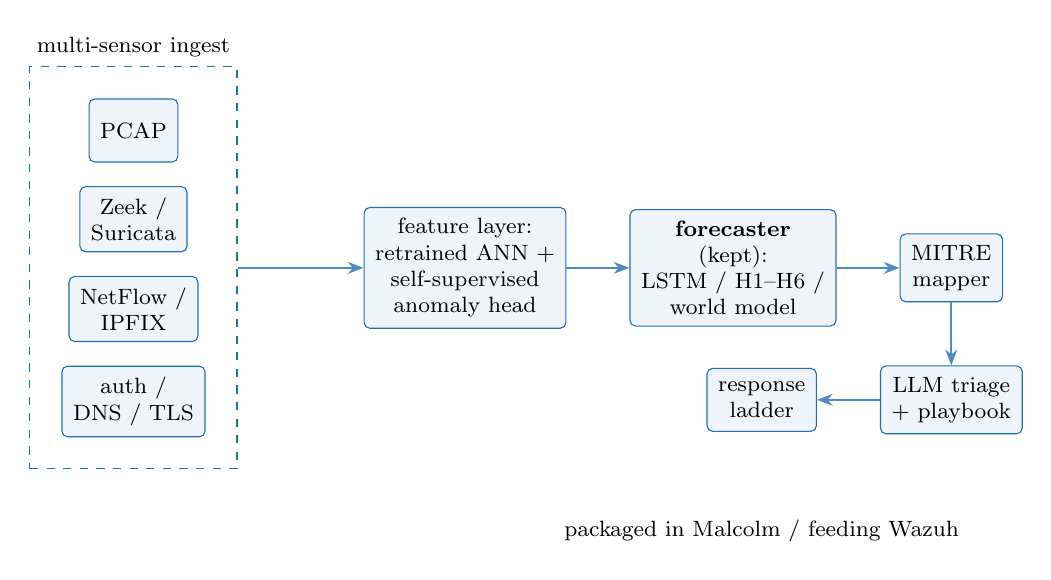
\begin{tikzpicture}[node distance=5mm and 8mm]
  \node[box] (s1) {PCAP};
  \node[box,below=3mm of s1] (s2) {Zeek /\\Suricata};
  \node[box,below=3mm of s2] (s3) {NetFlow /\\IPFIX};
  \node[box,below=3mm of s3] (s4) {auth /\\DNS / TLS};
  \begin{scope}[on background layer]
  \node[draw=accent,dashed,fit=(s1)(s4),inner sep=4mm,label=above:{\footnotesize multi-sensor ingest}] (S) {};
  \end{scope}
  \node[box,right=16mm of S] (feat) {feature layer:\\retrained ANN +\\self-supervised\\anomaly head};
  \node[box,right=of feat] (fc) {\textbf{forecaster}\\(kept):\\LSTM / H1--H6 /\\world model};
  \node[box,right=of fc] (mit) {MITRE\\mapper};
  \node[box,below=8mm of mit] (llm) {LLM triage\\+ playbook};
  \node[box,left=of llm] (resp) {response\\ladder};
  \draw[fl] (S)--(feat); \draw[fl] (feat)--(fc); \draw[fl] (fc)--(mit);
  \draw[fl] (mit)--(llm); \draw[fl] (llm)--(resp);
  \node[below=10mm of resp,font=\footnotesize,align=center] {packaged in Malcolm / feeding Wazuh};
\end{tikzpicture}
\caption{Target architecture. Coverage comes from adopting solved sensor/SIEM
pieces; the forecasting layer stays ours.}
\end{figure}

\clearpage
\part*{Part VI --- The roadmap}
\addcontentsline{toc}{section}{PART VI --- The roadmap}

\textbf{Stance: adopt the solved open-source pieces for coverage; keep the
forecaster as the thing that is genuinely new.} Steps in order.

\section{Step 1 --- Widen the front door}
Add a Zeek / Suricata / NetFlow ingester beside the PCAP path (or run the whole
pipeline as a \textbf{Slips module}). New \texttt{backend/ingest/} + a
\texttt{/api/ingest/} route. This alone removes the ``must run local packet
capture on the box'' limit --- the system then works on a span port or a
collector.

\section{Step 2 --- Refresh the detector}
Retrain the ANN on \textbf{NF-CSE-CIC-IDS2018-v2 / NF-UNSW-NB15-v2 /
CIC-IoT-2023} (NetFlow-format, labelled, same feature shape) and widen the label
set past four. Add a \textbf{self-supervised anomaly head} (autoencoder /
Isolation Forest / deep SVDD) on the current 77 features for unknown / zero-day
--- trains on benign traffic only, needs no new labels.

\section{Step 3 --- Track C: communication-graph GNN}
Hosts are nodes, flows are edges. Train a self-supervised link-prediction model
on benign traffic (E-GraphSAGE / Anomal-E style); score live edges by surprise.
New \texttt{backend/graph/} + \texttt{/api/graph/} + a \textbf{``Campaign''}
dashboard tab for lateral movement / botnet / APT. Trains on
NF-CSE-CIC-IDS2018-v2.

\begin{figure}[H]\centering
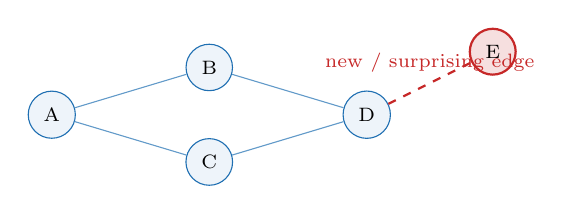
\begin{tikzpicture}[every node/.style={font=\scriptsize}]
  \node[circle,draw=accent,fill=soft] (a) at (0,0) {A};
  \node[circle,draw=accent,fill=soft] (b) at (2,0.6) {B};
  \node[circle,draw=accent,fill=soft] (c) at (2,-0.6) {C};
  \node[circle,draw=accent,fill=soft] (d) at (4,0) {D};
  \node[circle,draw=bad,fill=bad!15,thick] (e) at (5.6,0.8) {E};
  \draw[accent!70] (a)--(b); \draw[accent!70] (a)--(c); \draw[accent!70] (b)--(d); \draw[accent!70] (c)--(d);
  \draw[bad,thick,dashed] (d)--(e) node[midway,above,text=bad]{new / surprising edge};
\end{tikzpicture}
\caption{Track C. Almost every multi-stage attack shows up as a new or
surprising edge in the host graph before it shows up in any single flow.}
\end{figure}

\section{Step 4 --- Tracks E + G: real-time forecasting + LLM triage}
Replace ``row-order proxy seconds'' with real timestamps. Add a
\textbf{time-to-attack} survival / hazard head (``attack within T minutes:
p'') and a Hawkes point-process for attack arrival, beside the world model. Add
a \textbf{local security-LLM panel} (Foundation-Sec-8B style) on top of
\texttt{mitre/mapper.py}: summarise an alert, rank techniques, draft a playbook,
explain ``why flagged'', correlate threat intel. Advisory only --- it never
writes a rule.

\section{Step 5 --- Tracks H + I: deception + graduated response}
\textbf{Deception:} a few honeypot services + honey-tokens (fake credentials,
fake share). Any interaction is a near-zero-false-positive label \emph{and} an
early-warning event; it feeds steps 2--4.

\textbf{Graduated response}, building on the \texttt{config.json}
\texttt{response.protected\_addresses} allow-list already added:

\begin{figure}[H]\centering
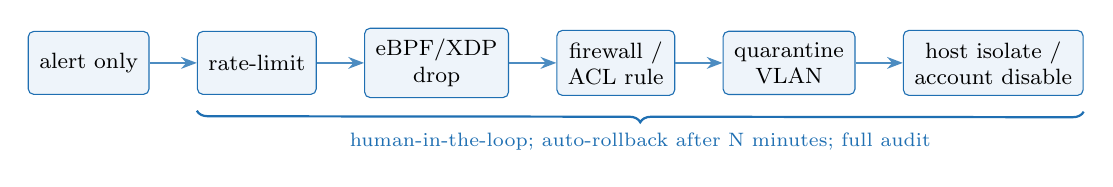
\begin{tikzpicture}[node distance=4mm]
  \node[box] (a) {alert only};
  \node[box,right=6mm of a] (b) {rate-limit};
  \node[box,right=6mm of b] (c) {eBPF/XDP\\drop};
  \node[box,right=6mm of c] (d) {firewall /\\ACL rule};
  \node[box,right=6mm of d] (e) {quarantine\\VLAN};
  \node[box,right=6mm of e] (f) {host isolate /\\account disable};
  \draw[fl] (a)--(b); \draw[fl] (b)--(c); \draw[fl] (c)--(d); \draw[fl] (d)--(e); \draw[fl] (e)--(f);
  \draw[decorate,decoration={brace,amplitude=4pt,mirror},thick,accent]
    ($(b.south west)+(0,-2mm)$) -- ($(f.south east)+(0,-2mm)$)
    node[midway,below=4pt,font=\scriptsize]{human-in-the-loop; auto-rollback after N minutes; full audit};
\end{tikzpicture}
\caption{Track I. Escalation is gated: anything above rate-limit needs an
operator, every action is logged, and everything rolls back on a timer.}
\end{figure}

\section{Step 6 --- Package for enterprise}
Ship the detector + forecaster inside \textbf{Malcolm}; feed \textbf{Wazuh} for
correlation and response; keep this dashboard as the analyst console.

\section{What this is not}
Steps stay honest about scope: the forecaster is short-horizon and window-based
until step 4; the graph and anomaly models need the modern datasets from step 2;
response actions above ``alert'' are operator-gated. Nothing here sends traffic
off the box.

\clearpage
\part*{Part VII --- From NIDS to XDR}
\addcontentsline{toc}{section}{PART VII --- From NIDS to XDR}

\section{Why PCAP alone is blind}

PCAP is often called the ultimate source of truth --- it records exactly what
crossed the wire. Two realities bottleneck it against a modern threat matrix:

\begin{itemize}
\item \textbf{Ubiquitous encryption.} Ten years ago most web-app attacks (SQLi,
  XSS), phishing payloads and C2 beacons were cleartext, so payload inspection
  worked. Today over 90\% of traffic is encrypted. If an attacker downloads a
  living-off-the-land binary or brute-forces an HTTPS login, PCAP sees only a
  TLS stream between two IPs --- it cannot tell a Cobalt Strike payload from a
  PDF download.
\item \textbf{Visibility scope.} A tap or span port only sees the traffic on
  \emph{its} segment. Endpoint actions, identity events and wireless activity
  never cross it.
\end{itemize}

\begin{table}[H]\centering\small
\begin{tabular}{@{}p{2.6cm}p{5.4cm}p{6.3cm}@{}}
\toprule
\textbf{Visibility} & \textbf{Attack types} & \textbf{Why PCAP succeeds or fails} \\
\midrule
\textbf{High} (directly captured) & DoS/DDoS, port scans, DNS attacks, spoofing,
  IoT/OT, protocol evasion & these manipulate L3/L4 headers, flow rates, or use
  unencrypted protocols (DNS, Telnet, Modbus). PCAP is irrefutable ground truth. \\
\textbf{Partial} (behavioural / metadata) & malware C2, lateral movement,
  ransomware, exfiltration, cryptojacking & payloads are encrypted. PCAP must
  rely on metadata: flow volume, timing (beacon jitter), TLS handshakes
  (JA3/JA4/SNI), byte asymmetry. \\
\textbf{Low} (needs integrations) & phishing, brute force, web-app attacks,
  insider threat, LOLBins, wireless & activity is inside encrypted tunnels, on
  the endpoint (EDR), in auth systems (AD), or over the air (WIPS). Standard PCAP
  is blind. \\
\bottomrule
\end{tabular}
\caption{Attack-visibility breakdown. NIDS today lives in the ``High'' row plus
the metadata half of ``Partial''.}
\end{table}

\section{The SOC Visibility Triad + XDR fusion}

When PCAP is blinded, move the detection boundary to where data is either
unencrypted or actively executing. Four additions:

\begin{itemize}
\item \textbf{Endpoint telemetry (EDR / Sysmon)} --- catches ransomware,
  zero-days, LOLBins. Sees the action before encryption wraps it: process
  lineage (Word spawns a hidden PowerShell that makes an outbound connection),
  credential-theft attempts against LSASS, and host-level networking that ties a
  connection back to the exact process that made it.
\item \textbf{Identity / authentication logs (AD / IAM)} --- catches lateral
  movement, insider threats, brute force. Track the credential, not the packet:
  Windows Event 4624 (network logon) with 4688 (process creation) --- one user
  account logging into 15 servers via SMB in five minutes is a red flag;
  Kerberoasting shows as unusual SPN ticket requests; ``impossible travel'' from
  a cloud IdP.
\item \textbf{Layer-7 proxies and WAF (AppSec)} --- catches web-app attacks and
  exfiltration. A WAF holds the TLS certificate, decrypts inbound HTTPS, inspects
  the raw payload for SQLi / path traversal, and blocks. A secure web gateway
  decrypts \emph{outbound} traffic and inspects it for C2 beaconing, phishing
  domains and data exfiltration before it leaves.
\item \textbf{XDR data fusion (behavioural analytics)} --- no single alert is
  enough for a low-and-slow campaign. Baseline what a service account normally
  does; if it connects to a new segment (NetFlow), uses a rare administrative
  share (EDR/Sysmon) and authenticates out of hours (identity), the platform
  fuses those low-confidence anomalies into one high-confidence ``campaign in
  progress'' alert.
\end{itemize}

\section{The architecture --- six tiers}

\begin{figure}[H]\centering
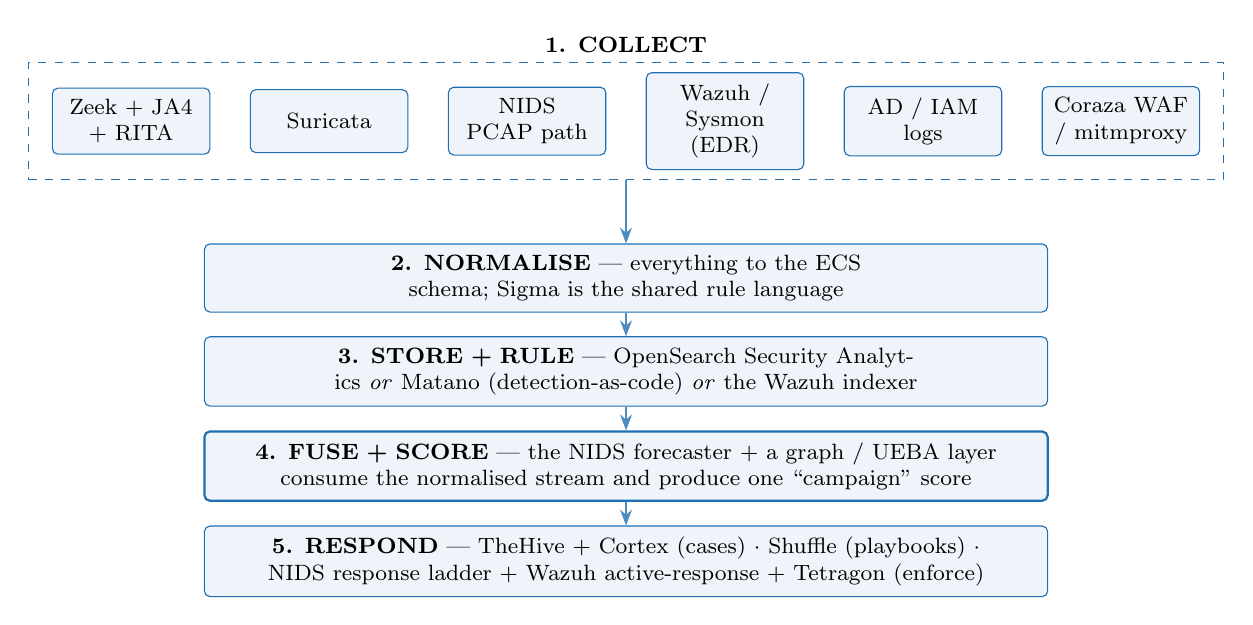
\begin{tikzpicture}[node distance=3mm and 5mm,every node/.style={font=\scriptsize}]
  \node[box,minimum width=20mm] (c1) {Zeek + JA4\\+ RITA};
  \node[box,minimum width=20mm,right=of c1] (c2) {Suricata};
  \node[box,minimum width=20mm,right=of c2] (c3) {NIDS\\PCAP path};
  \node[box,minimum width=20mm,right=of c3] (c4) {Wazuh /\\Sysmon\\(EDR)};
  \node[box,minimum width=20mm,right=of c4] (c5) {AD / IAM\\logs};
  \node[box,minimum width=20mm,right=of c5] (c6) {Coraza WAF\\/ mitmproxy};
  \begin{scope}[on background layer]
  \node[draw=accent,dashed,fit=(c1)(c6),inner sep=3mm,label={[font=\footnotesize]above:\textbf{1. COLLECT}}] (C) {};
  \end{scope}
  \node[box,below=8mm of C,text width=0.86\linewidth] (N) {\textbf{2. NORMALISE} --- everything to the ECS schema; Sigma is the shared rule language};
  \node[box,below=3mm of N,text width=0.86\linewidth] (S) {\textbf{3. STORE + RULE} --- OpenSearch Security Analytics \emph{or} Matano (detection-as-code) \emph{or} the Wazuh indexer};
  \node[box,below=3mm of S,text width=0.86\linewidth,fill=soft,draw=accent,thick] (F) {\textbf{4. FUSE + SCORE} --- the NIDS forecaster + a graph / UEBA layer consume the normalised stream and produce one ``campaign'' score};
  \node[box,below=3mm of F,text width=0.86\linewidth] (R) {\textbf{5. RESPOND} --- TheHive + Cortex (cases) $\cdot$ Shuffle (playbooks) $\cdot$ NIDS response ladder + Wazuh active-response + Tetragon (enforce)};
  \draw[fl] (C)--(N); \draw[fl] (N)--(S); \draw[fl] (S)--(F); \draw[fl] (F)--(R);
\end{tikzpicture}
\caption{NIDS stays the network sensor and the forecasting brain (tier 4). The
Triad adds three more collection streams; a normalise + store layer gives one
schema; response is a dedicated tier.}
\end{figure}

\section{What to install --- open-source tools, and where each plugs into NIDS}

\begin{longtable}{@{}p{2.7cm}p{4.6cm}p{6.6cm}@{}}
\toprule
\textbf{Triad layer} & \textbf{Tool (GitHub)} & \textbf{Adds / integration point} \\
\midrule \endhead \bottomrule \endfoot
Network metadata & \texttt{zeek/zeek} + \texttt{FoxIO-LLC/ja4} + \texttt{activecm/rita} &
  DNS / TLS / HTTP / SMB / SSH logs; JA4 fingerprints; per-pair beacon score
  0--1. New \texttt{backend/ingest/zeek} + \texttt{/api/ingest/zeek}; feed the
  fields + JA4 + beacon score into the 28-number window state; a ``Campaign /
  C2'' tier beside \texttt{signatures.py}. \\
Signature IDS & \texttt{OISF/suricata} + ET Open rules & protocol anomalies,
  known-bad, JA3. Alerts into the fusion store; a signature tier alongside the
  existing rule layer. \\
Endpoint (EDR) & \texttt{wazuh/wazuh} agents + Sysmon
  (\texttt{SwiftOnSecurity/sysmon-config} or \texttt{olafhartong/sysmon-modular}) &
  process lineage, LSASS-access blocks, host netconn$\leftrightarrow$process.
  Correlate a NIDS network verdict with the exact process that caused it. \\
Host forensics & \texttt{Velocidex/velociraptor} \emph{or}
  \texttt{osquery/osquery} + \texttt{fleetdm/fleet} & on-demand ``what happened
  on this host?'' hunts, triggered from a case. \\
Identity / auth & Windows 4624 / 4688 / 4769 via Wazuh or \texttt{elastic/beats}
  (Winlogbeat); \texttt{SigmaHQ/sigma}; \texttt{wagga40/Zircolite} &
  lateral-movement velocity, Kerberoasting SPN requests, impossible travel.
  Auth-velocity + lateral-graph features feed the forecaster. \\
L7 inbound (WAF) & \texttt{corazawaf/coraza} (Go, OWASP, active) \emph{or}
  \texttt{chaitin/safeline} \emph{or} \texttt{bunkerity/bunkerweb} +
  \texttt{coreruleset/coreruleset} & terminate inbound HTTPS, inspect payload for
  SQLi / XSS / traversal, block. WAF alerts into fusion; a block is a NIDS
  \emph{prevent} action. \\
L7 egress (SWG / DLP) & \texttt{mitmproxy/mitmproxy} \emph{or} Squid + SSL-bump
  \emph{or} BunkerWeb as egress proxy & decrypt egress $\rightarrow$ see C2
  beacons, phishing domains, data exfiltration. Decrypted egress metadata into
  the same window features. \\
Fusion / SIEM & \texttt{opensearch-project/security-analytics} \emph{or}
  \texttt{matanolabs/matano} (Python detection-as-code, auto-imports Sigma)
  \emph{or} the Wazuh indexer & one store, ECS schema, correlation. The fused
  stream is the forecaster's new input. \\
Cases + SOAR & \texttt{TheHive-Project/TheHive} + \texttt{TheHive-Project/Cortex}
  + \texttt{Shuffle/Shuffle} (or \texttt{n8n-io/n8n}) & a NIDS ATTACK verdict
  opens a case with the forecast + MITRE map attached; automated IOC enrichment;
  response playbooks. \\
Enforcement & Wazuh active-response; \texttt{cilium/tetragon} (in-kernel
  block / kill) & the top rungs of the NIDS response ladder. \\
\end{longtable}

\section{XDR-in-a-box --- if you want less assembly}

\begin{itemize}
\item \textbf{\texttt{Security-Onion-Solutions/securityonion}} --- Zeek +
  Suricata + Elastic + TheHive + Sigma + Playbook in one distribution. Closest
  thing to open-source XDR you can deploy in a day.
\item \textbf{\texttt{idaholab/Malcolm}} --- Zeek + Suricata + Arkime +
  OpenSearch, dockerised, OT-aware (CISA + Idaho National Lab). Best if you want
  to \emph{embed the NIDS forecaster} rather than adopt a whole SOC.
\item \textbf{\texttt{wazuh/wazuh}} --- already an XDR + SIEM in one
  agent / manager / dashboard; the fastest path to endpoint + identity + file
  integrity + active response.
\end{itemize}

All of the above are maintained by real organisations --- CNCF (Tetragon), OWASP
(Coraza, Core Rule Set), OISF (Suricata), the Zeek project, FoxIO (JA4), Chaitin
(SafeLine), Active Countermeasures / SsoT (RITA), Wazuh Inc., Idaho National Lab
(Malcolm), StrangeBee (TheHive). Licences are Apache-2.0 / GPL / BSD.

\section{The smallest first step for this repo}

Add a \textbf{Zeek + JA4 + RITA sidecar} reading the same span port the PCAP path
already uses. Pipe \texttt{conn.log} / \texttt{ssl.log} / \texttt{dns.log} and
the RITA beacon score into the temporal window features. That one bolt-on lifts
C2, exfiltration, DNS-tunnelling and TLS-attack coverage from ``Low'' to
``Partial / High'' --- with \emph{no} endpoint-agent rollout and no change to the
capture path.

\clearpage
\part*{Appendices}
\addcontentsline{toc}{section}{Appendices}

\section*{Appendix A --- Glossary for a non-technical reader}
\addcontentsline{toc}{subsection}{Appendix A --- Glossary}
\begin{description}[leftmargin=3.2cm,style=nextline]
\item[Flow] one two-way conversation between two computers, identified by source
  and destination IP and port plus protocol.
\item[Feature] one number describing a flow (e.g.\ ``bytes per second'').
\item[Softmax] a model output that turns raw scores into probabilities that sum
  to 1.
\item[Confidence] the largest of those probabilities --- how sure the model is.
\item[Window] a fixed 10-second slice of time; all flows in it are summarised
  into one row.
\item[Sequence] five consecutive windows used as input to predict the sixth.
\item[Leakage] when information from the test period sneaks into training,
  making results look better than they are; the audit hunts for it.
\item[Macro-F1] an accuracy-like score that weights every class equally, so rare
  attacks count as much as common benign traffic.
\item[False-positive rate] the share of benign traffic wrongly flagged.
\item[Beaconing] malware ``phoning home'' at regular intervals.
\item[Lateral movement] an attacker hopping from the first compromised machine
  to others inside the network.
\item[GNN (graph neural network)] a model that learns from a network of
  connections rather than a flat table.
\item[Self-supervised] trained on unlabelled ``normal'' data; anything unlike
  normal scores as anomalous.
\item[Foundation model] a large model pretrained on huge unlabelled data, then
  fine-tuned for a specific job with little labelled data.
\item[MITRE ATT\&CK] a public catalogue of attacker techniques, each with an ID
  like T1595.
\item[Kill chain] the stages of an intrusion, from reconnaissance to impact.
\end{description}

\section*{Appendix B --- Key numbers}
\addcontentsline{toc}{subsection}{Appendix B --- Key numbers}
\begin{longtable}{@{}p{7cm}p{7cm}@{}}
\toprule \textbf{Name} & \textbf{Value} \\ \midrule \endhead \bottomrule \endfoot
Class names / softmax order & BENIGN, DDoS, DoS, PortScan \\
Flow feature count & 77 \\
State-vector size (temporal) & 28 \\
Unscoreable sentinel & INVALID\_FEATURES \\
Write-back columns & Current\_State, Signature\_State, Effective\_State \\
Verdict gate (DDoS / other) & own-class share $\geq$ 20\% / 20\% \\
Capture default duration & 300 s \\
Capture safety timeout & 600 s \\
Capture buffer & 64 MiB \\
Parallel-extract chunk / threshold & 20\,000 / 20\,000 packets \\
Signature DDoS fan-in / pkts-s / victim-ratio / top-source & 20 / 100 / 0.5 / 0.25 \\
Signature DoS SYN / ACK-ratio / pkts-s & 20 / 0.2 / 100 \\
Signature PortScan ports / max fwd bytes & 20 / 400 \\
Window length / sequence length & 10 s / 5 \\
Chronological split & 70 / 15 / 15 \\
One-step LSTM & LSTM(64) -> Dense(32) -> 2 x softmax(4); seed 42; max 40 epochs; batch 512 \\
Multi-step horizons K & 6 (direct) \\
World model K & 6 default, 24 max; hidden 64; early-warning 0.60 \\
Early-warning threshold selection & max attack-F1 s.t.\ FPR $\leq$ 5\% \\
MITRE techniques covered & T1595, T1046, T1498(.001/.002), T1499 (ATT\&CK v19.1) \\
Mapping confidence values & 0.25 / 0.55 / 0.65 (heuristic, not calibrated) \\
Active LSTM model & v1-3a5264a499ed \\
\end{longtable}

\section*{Appendix C --- Sources}
\addcontentsline{toc}{subsection}{Appendix C --- Sources}
\small
India incidents: Kudankulam --- VIF analysis; Gulf News. AIIMS --- ORF; RingSafe;
CM-Alliance timeline. Cosmos Bank --- Securonix threat research; Indiaforensic.
RedEcho / power --- Outlook; Eventus. Hacktivist DDoS --- GovInsider; SecurityLink
India; CERT-In advisory CIAD-2023-0036.

Research: NetFlow context deep-learning survey (arXiv 2602.05594); FastFlow
(arXiv 2504.02174); encrypted HTTPS stacked ensembles (Nature s41598-025-21261-6);
encrypted malicious traffic NLP+DL (ScienceDirect S1389128624004304); E-GraphSAGE
(arXiv 2103.16329); GNN-IDS survey (Computers \& Security 2024,
10.1016/j.cose.2024.103821); graph foundation model for lateral movement
(arXiv 2504.13527); heterogeneous-graph cyber anomaly survey (arXiv 2510.26307);
ML cybercrime prediction review (arXiv 2304.04819); forecasting cyber threats +
mitigation (ScienceDirect S0040162524006346); forecasting from incomplete data
(arXiv 2004.04597); eBPF/XDP DDoS mitigation (arXiv 2508.00851); eBPF DoS
detection in Kubernetes (MDPI Applied Sciences 13/8/4700); netFound
(arXiv 2310.17025); NetMamba (arXiv 2405.11449); Anomal-E (arXiv 2207.06819).

Open source (Parts V--VI): github.com/stratosphereips/StratosphereLinuxIPS;
github.com/idaholab/Malcolm; github.com/arkime/arkime; github.com/wazuh/wazuh;
github.com/zeek/zeek; github.com/OISF/suricata; github.com/linwhitehat/et-bert;
github.com/wangtz19/Awesome-NTA; github.com/zhadyz/AI\_SOC;
github.com/scadastrangelove/awesome-ai-security-tools; Cisco Foundation-Sec-8B.

XDR / SOC Visibility Triad (Part VII): github.com/Velocidex/velociraptor;
github.com/osquery/osquery; github.com/fleetdm/fleet; github.com/FoxIO-LLC/ja4
(``How to Use JA4 Network Fingerprints in Zeek'', zeek.org, Jan 2026);
github.com/activecm/rita (Active Countermeasures / SsoT); github.com/corazawaf/coraza;
github.com/chaitin/safeline; github.com/bunkerity/bunkerweb;
github.com/coreruleset/coreruleset; github.com/mitmproxy/mitmproxy;
github.com/SigmaHQ/sigma; github.com/wagga40/Zircolite;
github.com/opensearch-project/security-analytics; github.com/matanolabs/matano;
github.com/TheHive-Project/TheHive; github.com/TheHive-Project/Cortex;
github.com/Shuffle/Shuffle; github.com/cilium/tetragon;
github.com/Security-Onion-Solutions/securityonion;
github.com/SwiftOnSecurity/sysmon-config; github.com/olafhartong/sysmon-modular.
Reviews: packetlabs.net open-source EDR; pistack.xyz Wazuh vs Velociraptor vs
osquery 2026; manageengine / exabeam open-source SIEM 2026; wafplanet.com
Coraza / SafeLine / BunkerWeb 2026; blackhillsinfosec.com ``Detecting Malware
Beacons with Zeek and RITA''.

\end{document}
